% UCSD Mathematics Dissertation Template
%
% Please read the comments in this file and make appropriate edits.
% NOTE: Always refer to the ``Preperation and Submission Manual for 
% Doctoral Dissertations and Masters Theses for 20**'', where 20** is 
% the year of your graduation, for officiation preparations guidelines.
%
% If you desire more control, please see the attached files:
%   * ucsd.cls -- Class file
%   * uct10.clo, uct11.clo, uct12.clo -- Configuration files for font sizes 10pt,11pt,12pt
%
% CHANGELOG:
%   * Original file adapted from brockman.tex by JRB and RMR
%     to work with ucsd.cls


\documentclass[12pt,chapterheads]{ucsd}
% documentclass options: default is 11pt, oneside, final.
% fonts: 10pt, 11pt, 12pt -- are valid for UCSD dissertations.
% sides: oneside, twoside -- note that two-sided theses are not accepted by OGS
% mode: draft, final -- draft mode switches to single spacing, removes hyperlinks,
%                       and places a black box at every overfull hbox (check these before submission).
% chapterheads -- include this if you want your chapters to read:
% Chapter 1
% Title of Chapter
%
% instead of
%
% 1 Title of Chapter


% Include all packages you need here.  Some standard options are suggested below.

% GEOMETRY - This will force the use of Letter paper.
% Many TeX installations default to A4 paper.  The formatting
% of the thesis class file requires Letter, else the margins
% will be wrong when you go to print it (and OGS will complain).
% If your TeX implementation is not setup for Letter paper, and
% you cannot change it, uncommenting the following line may fix 
% problem.
\usepackage[paper=letterpaper]{geometry}

\usepackage{todonotes} %gzb
\usepackage{subcaption} %gzb
%\usepackage{titlesec}
\setcounter{tocdepth}{3}% Include \subsubsection in ToC

\usepackage[toc,page]{appendix}

%% AMS PACKAGES - Chances are you will want some or all of these if writing a math dissertation.
\usepackage{amsmath, amscd, amssymb, amsthm}

%% GRAPHICX - This is the standard package for including graphics for latex/pdflatex.
\usepackage{graphicx}

%I tend to use double quotes the "traditional way"
\usepackage [english]{babel}
\usepackage [autostyle, english = american]{csquotes}
\MakeOuterQuote{"}

%\usepackage{caption}
%\usepackage{subcaption}

%% LATIN MODERN FONTS (replacements for Computer Modern)
% \usepackage{lmodern}
% \usepackage[T1]{fontenc}

%% INDEX
% Uncomment the following two lines to create an index: 
 \usepackage{makeidx}
 \makeindex
% You will need to uncomment the \printindex line near the
% bibliography to display the index.  Use the command
% \index{keyword} within the text to create an entry in the index
% for keyword.

%% HYPERLINKS
% To create a PDF with hyperlinks, you need to include the hyperref package.
% THIS HAS TO BE THE LAST PACKAGE INCLUDED!
% Note that the options plainpages=false and pdfpagelabels exist
% to fix indexing associated with having both (ii) and (2) as pages.
% Also, all links must be black according to OGS.
% See: http://www.tex.ac.uk/cgi-bin/texfaq2html?label=hyperdupdest
% Note: This may not work correctly with all DVI viewers (i.e. Yap breaks).

%hyperlinks package
\usepackage[colorlinks=true, pdfstartview=FitV, linkcolor=black, citecolor=black, urlcolor=black,plainpages=false,pdfpagelabels]{hyperref}

%metadata
\hypersetup{ pdfauthor = {Gabriel Zalles Ballivian}, pdftitle = {quals}, pdfkeywords = {music, audio, spatial}, pdfcreator = {pdfLaTeX with hyperref package}, pdfproducer = {pdfLaTeX}}

\begin{document}

%% REQUIRED FIELDS -- Replace with the values appropriate to you
\title{Spatial music: an open source approach}

% No symbols, formulas, superscripts, or Greek letters are allowed
% in your title.

\author{Gabriel Zalles Ballivian}
\degreeyear{2021}
\degree{Doctor of Philosophy} 
% Master's Degree theses will NOT be formatted properly with this
% file.

\field{Music}
\chair{Shahrokh Yadegari}
% Uncomment the next line iff you have a Co-Chair
% \cochair{Professor Cochair Semimaster} 
\othermembers{%  These must be alpha by last name.
Professor Erbe, Tom\\ 
Professor Smyth, Tamara\\
}
\numberofmembers{5} % |chair| + |cochair| + |othermembers|

\begin{frontmatter}
\makefrontmatter % The title, copyright, and signature pages.

%% DEDICATION
% You have three choices here:
%   1. Use the ``dedication'' environment.   Put in the text you want,
%   and you'll get a perfectly respectable dedication page.
%
%   2. Use the ``mydedication'' environment.  If you don't like the
%   formatting of option 1, use this environment and format things
%   however you wish.
%
%   3. If you don't want a dedication, it's not required.

% \begin{dedication} % The style file will format this for you.
%   To two.
% \end{dedication}

% \begin{mydedication} % You are responsible for formatting here.
%   \vspace{1in}
%   \begin{flushleft}
% 	To me.
%   \end{flushleft}
%   
%   \vspace{2in}
%   \begin{center}
% 	And you.
%   \end{center}
% 
%   \vspace{2in}
%   \begin{flushright}
% 	Which equals us.
%   \end{flushright}
% \end{mydedication}

%% EPIGRAPH
%  The same choices that applied to the dedication apply here.

% \begin{epigraph} % The style file will position the text for you.
%   \emph{The music is in the making.}\\
%   ---Miller Puckette
% \end{epigraph}

% \begin{myepigraph} % You position the text yourself.
%   \vfil
%   \begin{center}
%     {\bf Think! It ain't illegal yet.}
% 
% 	\emph{---George Clinton}
%   \end{center}
% \end{myepigraph}

\tableofcontents
\listoffigures  % Uncomment if you have any figures
\listoftables   % Uncomment if you have any tables

%% ACKNOWLEDGEMENTS
%  While technically optional, you probably have someone to thank.
%  Also, a paragraph acknowledging all coauthors and publishers (if
%  you have any) is required in the acknowledgements page and as the
%  last paragraph of text at the end of each respective chapter. See
%  the OGS Formatting Manual for more information.

\begin{acknowledgements} 
 Thanks for reading my answers.
\end{acknowledgements}


%% VITA
%  A brief vita is required in a doctoral thesis. See the OGS
%  Formatting Manual for more information.

\begin{vitapage}
\begin{vita}
  \item[2016] B.A. in Music, UC San Diego
  \item[2018] M.A. in Music, New York University
  \item[2023] Ph.D. in Music, UC San Diego (hopefully)
\end{vita}

\begin{publications}

    % only from start of phd. 
  \item Gabriel Zalles, ``Effects of Capsule Coincidence in FOA using MEMS: Objective Experiment'', \emph{AES147}, 2019.

\end{publications}

\end{vitapage}

%% Abstract
% There does not seem to be a maximum length. From the OGS Formatting
% Manual: ``The abstract may continue on to a second page.''

%Edited the ucsd.cls file. Abstract becomes questions from committee.

\begin{abstract}

\textbf{Question one (Tom Erbe):} what spatial instruments/pieces already exist? How has spatial music developed in the last 30 years? Are any of these instruments FOSS/FOSH? Propose some systems that one might employ for real-time spatial sound synthesis. What is novel about these?

\par
\vspace{2mm}

\textbf{Question two (Tamara Smyth):} how does one go about recording/capturing spatial music using FOSS? What techniques exist for this? What are the limitations today of these recording technologies? What other documentation/formats/files does one need to create? Beyond recording, how does FOSS aid in the ability of computer music composers to have their works survive technological shifts (changes in OS, protocols, etc.)?  

\par
\vspace{2mm}

\textbf{Question three (Shahrokh Yadegari):} once a spatial work is created and recorded, what open XR technologies exist that one can leverage to present their works? What are the technical difficulties associated with this kind of work? What are the artistic difficulties associated with this kind of work? What are the differences between WebXR, MobileXR and HMDs (or related technologies like CAVEs)? Be able to talk about the visual system in relation to XR.
  
\end{abstract}

\end{frontmatter}

%% DISSERTATION

% create -> record -> publish

% create live spatial music. CH2
% record the results in 3D audio. CH3
% publish with spatial attributes. CH4

%intro 
\chapter{Introduction} \label{ch:intro}

This document constitutes our efforts to organize a body of literature concerning the development of spatial music, spatial instruments, and systems relying on XR frameworks which can jointly be used for musical experiments. The focus of this work is to use Free and Open Source Software (FOSS) and low-cost solutions which might allow for greater proliferation of spatial music. In this work we will talk about the history of pioneering composers of \textit{spatial music} as well as what FOSS exists today for the creation, documentation and dissemination of these works.

In Chapter \ref{ch:intro} we will introduce the concept of spatial audio and focus primarily on the psycho-acoustic principles exploited in these works. We will also talk about the art, physics, and cognition of spatial audio, albeit briefly. Chapter \ref{ch:spat-mus} deals with spatial music and spatial instruments. Sometimes, although not always, spatial instruments are inextricably linked to a musical work, which is why we decided to use a single chapter to cover both of these topics. The chapter \ref{ch:spat-aud} talks about spatial audio capture and reproduction. We cover the history of these techniques, continue with an overview of state-of-the-art systems, and finally discuss some open-source solutions for both of these problems. Chapter \ref{ch:xr-mus} discusses how contemporary extended reality (XR) systems can be leveraged in order to expose more people to spatial music. We will talk about how some of these systems work, list some commercial solutions, and then discuss what FOSS exists for artists to present their works.

Each of these chapters has an associated proposal that connects with the material covered in the related chapters. These three proposals can be found in the appendix of this work. The chapters \ref{ch:intro} and  \ref{ch:conclusion} do not have associated proposals, since these are only contextual chapters. 

All of the figures in this body of work fall under the Creative Commons license. Any figures which do not have citation were created by the author and also fall under this designated category. We encourage the reader to use these figures for their own work. 

\todo[inline]{there are many different licenses. I have to go back and check what kind of licenses all these figures have. it would also be good to have an appendix that describes the different licenses for media and code since these are important to our work.}

\section{Physics of Sound}

%https://books.google.com.bo/books?id=OywDx9pxCMYC&pg=PA1&source=gbs_toc_r&hl=es-419#v=onepage&q&f=false

\section{Auditory System}

% https://commons.wikimedia.org/wiki/Ear#/media/File:Ear-anatomy.png

\section{Neurophysiology of Spatial Sound}
%http://cognet.mit.edu/book/auditory-neuroscience


\section{Art of Spatial Sound}

Space as a parameter of music-making is a feature which has been explored by composers for hundreds of years. Unfortunately, most musicians have a limited understanding of the possibilities that modern systems provide them and continue to operate on the basis of two-dimensional sound\footnote{Left/right panning plus distance modeled via amplitude changes or the addition of reverberation. A three-dimensional model would include height.}. Despite gargantuan efforts by the audio industry to expand commercial systems from stereo to more sophisticated formats, two-channel audio reproduction systems have remained the \textit{de facto} playback method in most homes due to their accessibility and simplicity. 

Before the rise of electro-acoustic composers, many artists experimented with space as a parameter of composition by including within their scores: the placement of musicians in different parts of the concert hall; choreographed trajectories for musicians; or using height by placing musicians in balconies. Many challenges that existed then remain now: synchronicity between players, architectural changes between venues, or, providing a consistent experience for all audience members regardless of their seat. 

Avant-garde composers in the 20th century pushed the envelope further by taking advantage of the technological developments of their era. With the advent of transmitted and recorded sound, \textit{disembodied sound} - a musicological term referring to the displacement in space-time of musician and sound - found a permanent role in the \textit{acousmatic}\footnote{Acousmatic generally means musical works where the musicians are not present. We only experience pre-recorded sounds in these types of works.} works of: Schaeffer, Xenakis, and Cage, to name a few. These acousmatic works, meant for reproduction over loudspeakers, made great use of spatial audio technologies such as the \textit{quadraphonic} or \textit{octophonic} sound systems\footnote{Four and eight channel sound systems, respectively.}, which were being developed at the time. 

Unfortunately, despite great scientific leaps, many of these older works cannot be fully appreciated by the general public since these high-end sound reproduction systems remain protected by privileged institutions. Commercial movie theatres, which harbor similar systems, have no financial incentive to reproduce these works. Part of the motivation of this thesis is to explore accessible techniques for the creation, documentation, and dissemination of works which employ spatial sound as a primary component of the compositional process. 

While many composers today, in well-funded contexts, have the pleasure to explore spatial sound through the use of multi-channel systems, much of their detailed work commonly gets \textit{down-mixed}\footnote{Compressed down from a multi-track format to stereo, usually for commercial purposes.} to stereo formats prior to distribution. If the spatial attributes of a particular sound are indeed important to the composition, this ultimate representation leaves much to be desired. %Luckily, many free and open-source solutions exist for audio engineers to create and re-distribute works of this variety preserving the environmental auditory elements pertinent to the works. 

In addition to discussing technologies available for the creation, recording, and presentation of 3D audio - in a musical context - we will discuss some of the technical challenges inherent in these productions. Namely, we will consider the difficulty of 3D sound reproduction based on computer: storage, speed, and changing operating systems (OS). We hope this work proves useful for any composer interested in the minutiae of the science, and art, of \textit{spatial music}.

\section{Psycho-acoustics of Spatial Sound}

Before we can understand the mathematical details behind different 3D audio technologies\footnote{3D audio is another name given to the field of spatial audio. In musical domain we often refer to this practice as sound \textit{diffusion}.}, we should discuss some of the psycho-acoustic principles on which all spatial audio technologies rely. Many authors have written extensively about the subject, with entire books having been dedicated to the subject - Blauert's 1997 \cite{blauert1997spatial} being perhaps the most popular. Here we will give only a short account of the many experiments that have been undertaken in this domain in order to inform the reader of some of the most salient features of the auditory system which inform our perception of sounds.

From the psycho-acoustic perspective, the most important feature of the auditory system is our ability to localize sound. This is perhaps why so much attention has been devoted to the subject in the psycho-acoustic community. Having a sensitive auditory localization system poses an evolutionary advantage; being able to detect the presence of a predator, before it can reach us, is likely why we have developed the ability to localize sound. Similarly, being able to detect prey, before it can escape, could be evolutionarily advantageous. 

A number of perceptual mechanisms work in conjunction, and amalgamate into a single sensory experience, informing our understanding of sound origins (directionally speaking). Not only are we conditioned to use acoustic cues to draw these conclusions, but memory and vision also form a part of this complex model \cite{kendall19953}. Our subconscious contains a mental map of the prevailing origin of different sounds based on prior experience which informs our predictions of source provenance. 

For example: we seldom hear birds chirping below us because they generally fly above our heads, or rest on branches that are higher than us. As a result, you will seldom see a bird-watcher searching for a particular species below them. They can safely assume the sound they hear comes from above, even if they are not sure. Furthermore, if they momentarily perceive that same bird to indeed be below them, for whatever reason, they will likely confirm or refute this suspicion by looking in that direction, and adapt their prediction based on the confluence of sensory information. 

Our auditory model of sound localization is quite complex, especially for multiple sources in spaces. When sound waves travel through air, if there is more than a single source, the pressure waves constructively and destructively interfere, making position estimations harder. Additionally, if the space is very \textit{reverberant} - if there are many reflections from walls - such as in a chapel, these predictions might become even more complicated to make. Figure \ref{fig:cosine-wave} shows a depiction of a cosine wave advanced in time, modified to show nodes and antinodes. Constructive and destructive interference refers to pressure waves' ability to increase or decrease in amplitude based on interactions with each other. For example, a negative pressure antinode might perfectly cancel a positive pressure antinode when two waves of equal frequency are offset in phase by 180\textdegree.

\begin{figure}[ht!]%force figure here, top, strict
\centering
\includegraphics[width=0.8\textwidth]{img/cosine-wave.png} 
%\captionsetup{justification=centering}
\caption{Cosine Wave \cite{FileWave97:online}}
% attribution-share alike
\label{fig:cosine-wave}
\end{figure}

It is useful within this scope to distinguish between source localization of \textit{near-field} and \textit{far-field} sources. As their names suggest, near-field sources are those that are proximal and far-field sources are those which are relatively distant from us. These definitions have real world implications, namely, near-field sources will arrive at our ears before any reflections muddle our perception of sound direction arrival. In contrast, far-field sources, in the real world, will produce complex spectra, since reflections and direct sound will interact in unpredictable ways. 

It is useful to further define two common conditions for sounds sources: those in \textit{free-fields} and those in \textit{diffuse-fields}. Free-field refers to an environment in which there is no reverberation; in other words, there are no surfaces upon which the sound may reflect. This condition is seldom found in nature, however, \textit{anechoic chambers} - rooms with no echoes - such as the one in Figure \ref{fig:ibm-anechoic}, have been designed specifically with this characteristic in order to conduct acoustic experiments. 

In contrast, diffuse-field refers to a condition in which prominent reflections are present, ideally with equal energy arriving from all directions. In architectural acoustics, diffusion will often be introduced intentionally, such as in concert halls, in order to spread energy evenly across the entire listening space. In between these two extremes there exists a continuum of acoustic spaces, each with their own acoustic characteristics, such as the: \textit{reverberation time} of the room, or the shortest reflection path from a source to a subject - whether that be a person or a receiver. 

\begin{figure}[ht!]%force figure here, top, strict
\centering
\includegraphics[width=0.6\textwidth]{img/ibm-anechoic.jpg} 
%\captionsetup{justification=centering}
\caption{IBM Anechoic Chamber \cite{FileIBMA4:online}}
\label{fig:ibm-anechoic}
\end{figure}

\todo[inline]{RT60, room acoustics, relevant to microphone calibration project. windowing. IR measurements. diffuse-field equalization. etc.}

\subsection{HRIRs}\label{subsec:hrirs}

An important aspect of spatialization in the musical domain, in addition to horizontal and vertical direction of sounds, is the distance of the event in relation to listener. For these three critical localization parameters\footnote{These being: horizontal position, vertical position, and distance .} various associated auditory mechanisms exist in the acoustic domain which facilitate our ability to place sources in space. 

In \textit{near-field} conditions, \textit{auralization} systems - systems that seek to replicate natural phenomena via digital means - tend to model distance as an independent characteristic of directional acoustic propagation. A common definition of near-field, albeit informal, is: anything within arms reach, or between 0.5m and 1m (\cite{Betbeder.2017})\footnote{1-2m is the typical distance for HRTF measurements.}. The idea behind this formal separation of near and far field is to exploit "tricks" in sound system design which help simulate real-world acoustic conditions at a much lower computational cost. By analyzing real-world acoustic snapshots, taken with microphones as \textit{impulse responses} (IR), we can observe that many acoustic spaces exhibit similar behaviors, statistically speaking, in particular regions of their IRs. By exploiting these similarities, it is possible to build systems which require less computational power while performing the same functions of more "expensive" algorithms.

Any acoustic space can be considered a linear time-invariant (LTI) system\footnote{LTI systems are a classification of engineering systems which can be fully described by an impulse response \cite{LinearTi32:online}.} which can be characterised by a single IR much like any digital or analog filter. Subtle changes in air pressure as a function of temperature can affect sound propagation, but for all intents and purposes this theory holds true. Inside the near-field, the abundance or lack of reverberant sound, caused by reflections from surfaces, can contribute to our perception of sound distance. However, it is more common to model the diffuse-field/far-field attributes independently, and use a complimentary system, based on free-field/near-field techniques, for horizontal and vertical auralization.

Within our free/near field condition we are not concerned with IRs of a single omni-directional acoustic sensor - for spatialization systems - but rather with the analysis of two impulse responses; ideally captured at the listeners ears. For this purpose there exist various methodologies for capturing the aforementioned IRs commonly referred to as \textit{binaural impulse responses} (BIRs) or \textit{Head Related Impulse Responses} (HRIRs), in the time domain\footnote{When these are taken in diffuse-field conditions they are also sometimes called Binaural Room Impulse Responses (BRIRs). When a Fourier transform is applied to these IRs they are refer to as HRTFs, or Head-Related Transfer Functions}. The most common technique involves placing two small microphones, or \textit{in-ear} microphones, inside a persons ears, and taking snapshots at as many positions as possible by sending \textit{exponential sinusoidal sweeps}\footnote{One among various IR capture methods including: balloon pops, maximum length sequence (MLS), and linear sinusoidal sweeps.} (ESS) from speakers surrounding the listener. For more detailed analysis of the ESS method we refer the reader to \cite{farina2007advancements}.

The recordings are then \textit{de-convolved} in order to obtain the effect only of the listeners head and body on the two recordings as a function of direction. When the excitation signal is perfectly known, de-convolution yields an impulse response which captures the effects of the: room, speaker and microphone. A full-spectrum signal is required for a good IR to be obtained. We tend to use \textit{flat} frequency microphones and speakers, and an anechoic chamber, which has no response, to isolate the effects of head and torso on the incoming signals. 

\begin{figure}[ht!]%force figure here, top, strict
\centering
\includegraphics[width=0.3\textwidth]{img/sphere-png.png} 
%\captionsetup{justification=centering}
\caption{Sphere \cite{Spherewi43:online}}
\label{fig:sphere}
%license: attribution 3.0
\end{figure}

Figure \ref{fig:sphere} shows a spherical grid, included here to facilitate visualization of the proposed acoustic system. Consider a speaker at each intersection between two lines and a listener with \textit{in-ear} microphones in the center of the sphere. The acoustic sampling of the sphere, in the \textit{binaural} sense, will take place by sending an ESS from each speaker resulting in two IRs (one for each ear). This complete set of HRIRs, ideally taken in free-field conditions, such as inside an anechoic chamber, contain: time, level, and spectral differences, used by our auditory system to localize sound. \cite{zotkin2006fast} also showed it is possible to invert the microphone and speaker positions to more quickly capture HRTF sets. In their experiment a micro-speaker was placed at the subject's ear canal who was surrounded by a grid of microphones. The benefit of this method is one can capture all the impulse responses for the left ear at once, using a single ESS, then repeat the process for the right ear. Traditionally, HRTF measurements are extremely time consuming which makes personalized HRTFs unrealistic for most people.

Individual acoustic characteristics the HRIRs have been assigned specific names. \textit{Inter-aural level difference} (ILD) refers to the overall energy difference between the two IRs, \textit{inter-aural time difference} (ITD) refers to the time offset, or phase delay, between measurements. Based on the \textit{diffraction} and \textit{reflection} effects caused by the geometry of the human head, the HRIRs will also exhibit spectral differences, which can be used to discern directions in situations when ITDs and ILDs are not sufficient. Diffraction refers to sounds ability to bend around objects. This is especially true for low frequencies. Reflection refers to sounds ability to bounce off objects. This is especially true for high frequencies.

ILDs are typically caused by the \textit{shadowing effect} of the head and are therefore frequency dependent (\cite{cuevas20193d}). In other words, the ILD will be greater for higher frequencies since lower frequencies diffract, or bend, around the head, while high-frequencies reflect off the head. ITDs are a prominent localization cue at low frequencies and ILDs are the prominent localization cue for mid and high frequency. This concept is known as the \textit{Duplex Theory of Localization} and was proposed by Lord Rayleigh in 1907. 

\subsection{Localization Errors}

Many terms have been defined in the psyscho-acoustic community to describe common localization errors in auditory experiments. Our ability to localize sounds is greatly dependent on the nature of the acoustic environment, as well as the frequency content of the sound source. Also, we should remember that, in the real world, more often than not, multiple sound sources will be present at the same time - making localization tasks more difficult still.

\begin{figure}[ht!]%force figure here, top, strict
\centering
\includegraphics[width=0.5\textwidth]{img/azimuth-bir.png}
%\captionsetup{justification=centering}
\caption{Azimuth BIR Case Scenario}
\label{fig:azimuth-bir}
\end{figure}

In order to demonstrate some common localization errors, we present figure \ref{fig:azimuth-bir}. Consider positions 1 and 3 the figure. Clearly these two positions on the \textit{transverse} plane, otherwise known as the horizontal plane, have identical ILDs and ITDs since the distance from both positions to the subject's ears is identical. Therefore, the subject will only be able to rely on spectral differences to localize the impinging sound. Our outer ear, or \textit{pinna}\footnote{Also called the auricle in some medical textbooks.}, blocks high frequencies arriving from behind the listener acting as low-pass filters. The HRIRs capture all these time and frequency differences in order to simulate directionally-dependent sound propagation via \textit{convolution} of the associated IRs. 

In contrast, differentiating between positions 2 and 4 should be substantially easier, since we see that the ITD and ILD differences will compliment spectral changes giving us additional information. Assuming the subject is facing position 1, the distance between position 2 and the subjects right ear, the \textit{ipsilateral} ear\footnote{The ear closest to the source.}, will be smaller than the distance to the \textit{contralateral} ear\footnote{The ear furthest away from the source.}. Sound propagates in air at a rate of around 343 m/s and as it travels it loses energy due to friction between molecules according the inverse-square law\footnote{The inverse square law states that with every doubling of distance away from the sound source, the sound will be four times less intense.}. 

\begin{figure}[ht!]%force figure here, top, strict
\centering
\includegraphics[width=0.5\textwidth]{img/body-planes.jpg}
%\captionsetup{justification=centering}
\caption{Body Planes \cite{body_planes_pic}}
\label{fig:body-planes}
\end{figure}

This additional distance results in a time delay between IRs, as well as level differences. However small these differences might seem, they are crucial for discerning the position of sounds in space. The inability of listeners to differentiate between two sources with identical ITDs and ILDs, when two sources are mirrored over the coronal plane\footnote{Also called the frontal plane.}; is called \textit{front-back confusion}. The same principle applies to sources mirrored over the \textit{transverse plane}\footnote{Also called the horizontal plane.}, these errors are called \textit{up-down confusions}. Sources mirrored over the \textit{mid-sagittal}\footnote{Also known as the longitudinal or median plane.} should be easily discerned since ILDs and ITDs will be quite large. The human auditory system has been shown to be extremely sensitive. The ITD for a typical human head can vary between $\pm$750$\mu$s. Humans can detect ITDs as low as 10-20$\mu$s which correspond to about 1\textdegree in the horizontal plane (\cite{hacihabiboglu2017perceptual}). 

\begin{figure}[ht!]%force figure here, top, strict
\centering
\includegraphics[width=0.5\textwidth]{img/cone_confusion.JPG}
%\captionsetup{justification=centering}
\caption{Cone of Confusion}
\label{fig:cone-confusion}
\end{figure}

The \textit{cone of confusion} is yet another term used to describe a common phenomenon experienced in localization experiments. Consider the two white dots on the circumference of the cone depicted in figure \ref{fig:cone-confusion}. The two positions, much like any two dots directly opposite each other on this circle, will have identical ITDs and ILDs because their respective distances to the \textit{contralateral} and \textit{ipsilateral} ears, will be the same. In this cases, spectral differences become critical to differentiate between sources. When ambiguous localization tasks arise, small head movements often help resolve source positions.

Our ability to localize sources is most accurate in the horizontal plane. Psycho-acoustic experiments have revealed that \textit{localization blur}, the inability for listeners to discern the direction of a sound, is generally less than 10\textdegree for horizontal sources, but around 20\textdegree for sources in the median plane (\cite{hacihabiboglu2017perceptual}). Two associated objective measures are the \textit{Minimum Audible Angle} (MAA) and the \textit{Minumum Audible Movement Angle} (MAMA). The MAA, a formal term used to quantify \textit{localization blur}, is the minimum detectable angular difference of two successive sound sources \cite{reardon2017evaluation}. The MAMA, is the smallest arc that a moving source must travel to be discriminable from a stationary source \cite{moore1995hearing}.

\subsection{Perception of Distance}

Perception of distance is more complex in some ways than that of orientation. \cite{zahorik2005auditory} provides, a comprehensive overview of auditory distance perception research, including some cognitive science research which examines brain response to acoustic stimuli. As aforementioned, there are several cues that affect our perception of distance - the most salient one being overall energy. A few other unmentioned cues, however, also affect our perception of distance. Among these is the absence or presence of high frequency content in a signal. High frequency signals tend to dissipate faster in air than low frequency ones, because of the additional friction between molecules inherent to these acoustic events. 

\textit{Auditory parallax}, the effect whereby the position or direction of an object appears to differ when heard from different positions, has also been shown to improve distance estimations. Finally, as mentioned before, familiarity tends to affect our perception of sound origin. A sample of a whispering voice, virtually placed far away, will appear closer than it really is. Adversely, a shouting voice, placed close, will appear to be further away than reality. It should be noted that this parallax is not limited to the subjects directional or rotational motion, the movement of the sound source can also help inform our perception of distance.

Finally, \textit{interaural coherence} (IC), is the measured statistical coherence of signals received at each ear. In a \textit{diffuse field}, IC is low, because the scattering of sounds off walls interact in unpredictable ways, which result in some amount of randomness in the signals when compared to each other. Therefore, IC can be used as a statistical estimate of distance, since we can assume that in most real-world conditions, sound sources will be diffused acoustically, lowering the overall IC for distant sources more than those proximal.

\subsection{Precedence Effect}

\textit{Summing localization} is a phenomenon - primarily based on ITD - which affects of perceived direction-of-arrival of sounds. When a broadband signal - a signal with broad range of frequencies present - is played from two directions with a delay of less than 1 ms, a single event is perceived at the direction between sources. The perceived location shifts towards the first played source, as the delay increases. This \textit{fusion} is one of three characteristics of the \textit{precedence effect}, also known as the \textit{Law of First Wavefront} or \textit{Haas effect}, described in 1949 by Helmut Haas. 

When the delay is between 1 and 5ms, a single event close to the leading source can be heard \cite{hacihabiboglu2017perceptual}. The lagging source - the delayed copy of the sound - can be perceived due to the change in timbre, and is perceptually equivalent to a feedforward comb filter where the delayed copy is played back over a second discrete channel. Within this context the \textit{echo threshold}, refers to the amount of delay that must be introduced to the copy before we begin perceiving the two sounds as independent non-fused events. This threshold is dependent on the nature of the signal. For a short broadband click, 5 ms might be enough to create an echo. For music and speech signals, the threshold is longer, and can be as high as 20 ms.

The precedence effect can be summarized by the following three phenomena: 

\todo[inline]{Each time I make a list I make the terms bold. I should make this standard throughout. Find "enumerate".}

\begin{enumerate}
    \item \textbf{Localization dominance}: the direction of an auditory event depends predominantly on the leading source.
    \item \textbf{Fusion}: a single auditory event is perceived when two sound events are below the \textit{echo threshold}.
    \item \textbf{Lag Discrimination Suppression}: the direction of the lagging sound is suppressed.  
\end{enumerate}

\subsection{Doppler Shift}

\textit{Doppler shift} is another auditory cue, related to \textit{auditory parallax}, which can aid in our estimation of source distance and direction. Doppler shift is the phenomenon we experience when we perceive the pitch of an ambulance's siren, or any other moving source, change as it approaches or moves away from us. Specifically, as the siren moves towards us, the pitch seems be higher than when stationary, and as it moves away, it seems to be lower than when stationary. This has to do with the nature of sound waves, which contract and expand in relation to the speed of the object. \cite{lavalle2016virtual} provides a whole chapter on the auditory mechanisms involved in Virtual Reality (VR). The book also covers the fundamentals of VR optics, interaction, and tracking, and is recommended for anybody interested in Extended Reality (XR). Equation \ref{eq:doppler}, from chapter 11, describes our perceived frequency of sound as a function of it's velocity. By combining this auditory cue with distance based intensity dampening we can realistically simulate moving sources.

\begin{equation}
f_{r}=\left(\frac{s+v_{r}}{s+v_{s}}\right) f_{s}
\label{eq:doppler}
\end{equation}

Where: 
\begin{enumerate}
    \item $f_r$ is the resulting frequency.
    \item $s$ is the speed of sound (343.2 m/s roughly at C 20\textdegree).
    \item $v_r$ is the velocity of the receiver (negative if receiver is moving away). 
    \item $v_s$ is the velocity of the source (negative is the source is moving away).
    \item $f_s$ is the original frequency of the source.
\end{enumerate}

\subsection{Binaural Synthesis Errors}

Of particular importance to our work is the use of binaural synthesis for the simulation of acoustic spaces. Binaural synthesis allows us to experiment with \textit{spatial music} without the need for sophisticated and often inaccessible loudspeaker systems. In binaural synthesis, sound sources are dynamically \textit{convolved}\footnote{Convolution of a source with an impulse response is equivalent to applying a filter.} with HRIRs to simulate surround sound experiences. Binaural synthesis has become increasingly popular with the growth of \textit{extended reality} (XR) systems. Several problems, such as: non-personalized HRTFs, externalization errors, and localization issues; persist. 

\todo[inline]{talk about non-personalized HRTFs and localization errors.}

Poor \textit{externalization}\footnote{Also sometimes referred to as Inside-the-Head Locatedness (IHL).}, the degree to which listeners perceive sources as originating inside their head, can be mitigated by the use of a head-tracking system. The systems, based on \textit{inertial measurement units} (IMU), monitor the orientation of the listener's head and adjusts the soundfield accordingly. When no rotation adjustment is included, our auditory system assumes that sources must be originating from inside our head, as this is the only rational conclusion for sources without dynamic filtering based on BIRs. The subtle spectral changes from location to location, provided by head-tracking, provide a way to disambiguate between source positions. The addition of diffuse field modeling, in the form of reverberation unit, also supports improved \textit{externalization}(\cite{sakamoto1976out}). 

\subsection{Reverberation}
%Room acoustics. T60, etc. Sabine equation. RT60. 

An important element of spatialization in virtual auditory environments (VAE) or in real-world environments is the reverberant characteristics of a space. Reverberation occurs when a dense network of echoes, with sufficiently small delay, mesh together to form a cohesive spatial image\footnote{The term spatial image used here to denote how the sound informs our perception of space.}. Sometimes the reverberation can be considered an obtrusive feature of a space, which reduces the intelligibility of the a signal. Other times, it can be deemed desirable, such as when musical events with harmonic relationships are performed in the reverberant space, this creating pleasing textures. 

Reverberation can provide the impression of realism, as sounds in space are seldom devoid of reverberation. It can also be pushed beyond the real towards artistic goals. Control over different characteristics of reverberation can be accomplished both in the architectural and digital domain. Since artists rarely have any control of architectural acoustics, and since this document is more closely concerned with computer-music approaches to spatialization, we will cover reverb processors from a software perspective. Some of the same principles, however, can be applied to architectural treatment of spaces. We refer the reader to \cite{gupta2019analysis} for a brief and concise overview of room acoustic design for recording studios. Finally, \cite{beranek1992concert} provides an overview of concert hall acoustics. 

\todo[inline]{I will come back to write this section. There is a lot to cover.}

\subsubsection{Algorithmic Reverbs}
\subsubsection{Convolution Reverbs}

\section{Conclusion}
This concludes our introduction to the subject of spatial sound. In this chapter we have presented the reader with different perspectives from which to begin appreciating the complexity of the field, and some background knowledge which should provide clarity to the proceeding chapters. Namely, we touched briefly on the compositional, psycho-acoustic and some of the engineering aspects of this domain. The next chapter will talk more in depth about the artistic practice of spatial sound drawing on historically important musical works, particularly in the field of electro-acoustic music. Chapter \ref{ch:spat-mus} will also talk about the development of spatial instruments which facilitate the creation of these works, and are sometimes indispensable to the recreation of these pieces.

%spatial music  (live) [CREATION]
\chapter{Spatial Music: Past, Present and Future}

\section{Introduction}

This chapter will be developed with Professor Tom Erbe. In this chapter we will discuss how spatial music has developed over the course of human history. We will talk briefly about some of the composers that broke ground by pioneering compositional techniques and then discuss modern approaches to spatial music by composers such as: Hagan, Lyon, Lopez-Lezcano, Barrett, and many more. 

We will also discuss spatial instruments, which refer to instruments which have considered the manipulation of sound in space as a critical parameter of the instrument design. In contrast to traditional instruments which assume sound radiates outwards from the acoustically activated object, these instruments might not produce any sounds by themselves and instead work in conjunction with computers, which receive data in order to synthesize sound at various real or \textit{phantom} speakers, also known as virtual speakers. 

These instruments are not always entirely electronic - at times we encounter designs in which "traditional" instruments have been extended via the use of sensors to give the performer control over the location of provenance of the sound. Often, computer musicians inextricably tie the development of instruments, or systems, to their compositions in ways that blur the line between: software and score, instrument and composition, or method and material. Some of these \textit{aesthetics} will also be discussed in this chapter. 

Finally, we would like to offer some speculative literature regarding what the likely direction of spatial music might be in the future. Spatial audio algorithms have been already thoroughly researched for many years. It appears on some level that many of the questions composers sought to ask regarding these systems have already been answered by these various developments. This final section will therefore consider how other technologies might be used in the future towards compositional means. 

\section{History of Spatial Music} \label{sec:hist_spat_mus}

This section will focus on the music from antiquity to the 21st century which uses space as a primary feature of the compositional process. In this chapter, we will trace the development of spatial music from its origins in the 4th century all the way to contemporary works. In future chapters we will seek to speculate how some of the most recent developments in systems design can contribute to this field. It is impossible to address all the works that have been created which fit our parameters, however, we will attempt to present the most important works in the field, as well as some attempts by the author himself to develop works in this space. 

\subsection{Acoustic Music} \label{subsec:acoustic_mus}

Our study of spatial music begins with the very earliest known examples of spatial compositions. \textit{Antiphonal} music is perhaps the oldest of these traditions. The practice of \textit{antiphonal} music, also known as "call and response", can be traced back to Biblical Times, with evidence of its existence as far back as the Roman Catholic Church in the 4th century. In a call and response system, the composer writes melodic lines using tension and resolution with independent choral group assigned different parts of the melody. The composer might create tension by using a dissonant note as the final note of the "calling" phrase. A different group, located in a different location of the stage, would resolve the melodic phrase, usually ending in the tonic of the scale and using some sort of traditional cadence. 

Many of these early works are hard to replicate today due to the lack of documentation. In the 16th century, however, printed works in spatial music would surface. Some of these initial innovative pieces were written by the Flemish composer Adrian Willaert\footnote{Netherlandish composer of the Renaissance.}, for example, whom exploited the \textit{Basilica de San Marco's\footnote{The cathedral church of the Roman Catholic Archdiocese of Venice, northern Italy.}} two organs in antiphonal compositions featuring two separate choirs and multiple instrumental groups \cite{arnold1959significance}. The technique \textit{cori spezzati}, or separated choirs, was re-introduced in his 1550's piece titled \textit{Vespers}, which itself featured multi-part arrangements and echo effect, likely in the form of a canon. Willaert's pupil, Andrea Gabrieli, an Italian composer of the late renaissance, would later continue his teacher's work, cementing spatial music as a hallmark of the Venetian musical practice. 

\begin{figure}[ht!]%force figure here, top, strict
\centering
\includegraphics[width=0.7\textwidth]{img/basilica-san-marcos.JPG} 
%\captionsetup{justification=centering}
\caption{Basilica de San Marco - wikimedia commons}
\end{figure}

As a result of Willaert's work the practice of spatial music quickly spread to other parts of Europe where it was quickly adopted by composers such as Thomas Tallis in England. \textit{Spem in alium}, one of Tallis's most famous pieces, was composed for Queen Elizabeth upon her 40th birthday, in 1573, and featured 40 vocal parts arranged in eight 5-voice choirs. The high point of spatial music during the baroque era might however be Orazio Benevoli's\footnote{Franco-Italian composer born in Rome (19 April 1605 – 17 June 1672).} \textit{Festival Mass}, written in 1628 for the \textit{Salzburg Cathedral} which called for 16 vocal parts, 34 instrumental parts, two organs, and a basso continuo\footnote{Figured bass where the most common combination is harpsichord and cello for chord and bass-line respectively.} \cite{zvonar1999history}.

Following the baroque era, interest in spatial music subsided until the beginning of the Romantic period. A key distinction of this era is the use of spatial music for theatrical effect, as the romantic period is often characterized by the rise and popularity of operas by composers such as: Hector Berlioz, a French Romantic composer and conductor (11 December 1803 – 8 March 1869) who wrote \textit{Requiem} in 1837, and Gustav Mahler, an Austro-Bohemian Romantic composer (7 July 1860 – 18 May 1911)\footnote{Considered one of the leading conductors of his generation.} who wrote \textit{Symphony No.2} in 1895 \cite{einstein1948music}. These composers not only spaced instruments for their performances but also choreographed the entrance and exiting of musicians as they played, creating some iconic musical moments.

In the 20th century, experimentalists such as Charles Ives, American modernist composer (October 20, 1874 – May 19, 1954), and Luigi Russolo, Italian Futurist composer and the author of the manifesto \textit{The Art of Noises} (30 April 1885 – 6 February 1947), who, inspired by the tumultuousness of industrial life, refined the art of musical collage using spatial sound \cite{jones199120th}. Ives's 1908 \textit{The Unanswered Question} called for offstage strings. Charles was inspired by his father George, a Civil War bandmaster, and music teacher, who had himself experimented with spatial music in his days. 

Henry Brant\footnote{Canadian-born American composer whom composed numerous orchestral spatial works (September 15, 1913 – April 26, 2008).}, inspired by Ives's music, would go on to create \textit{Antiphony I} (1953) which called for five spatially separated orchestras, and, \textit{Voyage Four} (1963) which called for three conductors to direct: percussion and brass on stage, violins on one balcony, violas and celli on another, basses on the floor level at rear, woodwinds at a rear balcony, and several performers in the audience \cite{zvonar1999history}. Brant's \textit{Windjammer} (1969), likely inspired by the opera composers of the baroque times, featured a static horn soloist and several wind players that moved along prescribed routes as they performed, in a choreographed manner. 

\cite{harley1997american} provides a rich analysis of four of Brant's most important works in the field of spatial music. Brant emphasized the need for differing timbres to be represented in his music, since he believed the heterogeneity would aid in the clarity of the musical representation. Indeed, if multiple instruments of the same family were spatially distributed, it would be difficult to differentiate melodic phrases, especially if these were all playing in the same register. Brant summarized his main observations with regards to spatial composition in a 1967 articles paraphrased as following: 

\begin{enumerate}
    \item \textit{Spatial separation clarifies texture}: when multiple musicians play different musical phrases in the same octave range, separating them spatially helps give clarity to each stream. 
    \item \textit{Separate groups are difficult to coordinate}: exact rhythms might be difficult to accomplish due to the distance it takes for sounds to arrive from one playing position to the next. 
    \item \textit{Spatial separation is equivalent to range separation}: it is possible to enhance the texture of a melodic phrase simply my separating musicians playing the same material.  
    \item Spatial arrangements must allow flexibility: the specific architectural demands of the works cannot always be met, alternatives should be provided whenever possible.
\end{enumerate}

Brant is perhaps one of the mos prolific composers of acoustic works with a repertoire of 67 spatial pieces. Brant also wrote extensively on the subject of spatial music and experimented at length with form, rhythm and perceptual experience. In contrast to other composers of his era, Brant's music dealt exclusively with acoustic means, which he creatively articulated to provide depth, envelopment and movement.  

\subsection{Electro-acoustic Music} \label{subsec:elec_acoustic_mus}

Along a parallel branch of history there exist a number of musical experiments conducted in the 20th century by avant-garde musicians and composers typically categorized as electro-acoustical. This label is used to separate them from traditional composers who avoided electronics or seldom exploited electronics in their compositions. The composers of this space and time were all activated by the development of sound recording, radio and telephony, and used them purposefully in their works. With the possibility of sound as a medium displaced from its source, dozens of new forms of music were created, this section will describe some. 

The birth of recorded sound brought with it an era of technological music development as composers and engineers sought to keep audiences attending live events - if only to see what strange machines were creating the sounds they could hear on their recordings at home. Thaddeus Cahill's \textit{Telharmonium} (1900-1906) is considered the first electrical musical instrument of its kind \cite{bode1984history}. Also known as the Dynamophone, this electrical organ was used to deliver music to homes on a subscription basis via a telephone line. We should note here that the element of space is present in an example such as this one, in a different semantic context, given the distance created between performer and audience. 

\begin{figure}[ht!]%force figure here, top, strict
\centering
\includegraphics[width=0.8\textwidth]{img/telharmonium.jpg} 
%\captionsetup{justification=centering}
\caption{Telharmonium Press - wikimedia commons}
\end{figure}

Later, in 1923, Leon Theremin would introduce a new instrument to the public. The theremin, named after its inventor, used two antennae to control the pitch and volume of a synthesizer. The user must position their hands in space to control the instrument and produce the desired sound. Theremin later formed ensembles in which multiple theremin were used in one of the first public displays of multi-channel loudspeaker music ever. The theremin is another particularly provoking example as it illustrates not only how space can be used for acoustic effect, but ergonomically speaking, it shows how an instrument can use space to facilitate its playing. Neither of these two instruments, however, exploit psycho-acoustic principles, the development of such instrument would come much later as we will see.  %spatial instrument

\begin{figure}[h!]%force figure here, strict
\centering
\includegraphics[width=0.5\textwidth]{img/theremin.jpg} 
%\captionsetup{justification=centering}
\caption{Alexandra Stepanoff\protect\footnotemark playing the theremin on NBC Radio, 1930 - wikimedia commons}
\end{figure}

\footnotetext{Alexandra Stepanoff was one of Léon Théremin’s first theremin students in the United States. Formerly a concert singer, around the late twenties, she moved from Russia to New York, where, thanks to the local Russian community, she met Léon Théremin.\cite{2020_stepanoff}}

The 20th century also saw the rise of phonographs\footnote{Colloquially known as record players.} as musical instruments. Paul Hindemith\footnote{Prolific German composer (16 November 1895 – 28 December 1963).} began this practice in the 1920's and 30's nearly 80 years before DJing practices became popular \cite{manning2013electronic}. John Cage\footnote{American avant-garde composer (September 5, 1912 – August 12, 1992).} also adopted the use of phonographs compositionally in \textit{Imaginary Landscape No. 1} (1939) which used multiple turntables and test tones, and in \textit{Imaginary Landscape No. 4} (1951) where he used 12 radios, 24 performers and a conductor. In addition to exploring the use of phonographs as instruments, Cage also exploited radio broadcast and tape in his creative practice.  

% \begin{figure}[ht!]%force figure here, top, strict
% \centering
% \includegraphics[width=0.5\textwidth]{img/phono.jpg} 
% %\captionsetup{justification=centering}
% \caption{Phonograph - \cite{cc}}
% \end{figure}

By separating the original performer from the playback these composers were playing not just with space, but also time. Cage, along with a group of experimental composers called "Project for Music for Magnetic Tape", would go on to write four pieces for tape \cite{cage1961experimental} during the 50s. The most famous piece that emerged from the group was likely \textit{William's Mix} (1952) which called for 8 tape machines each played back from its own speaker and thousands of snippets of sound carefully spliced together. The project also resulted in works by Earle Brown\footnote{American composer who pioneered the use of graphic scores (December 26, 1926 – July 2, 2002).} (\textit{Octet}) and Morton Feldman\footnote{American composer perhaps best known for his extended works which could last up to six hours (January 12, 1926 – September 3, 1987).} (\textit{Intersection}), both using 8 tape players and speakers. 

\begin{figure}[ht!]%force figure here, top, strict
\centering
\includegraphics[width=1.0\textwidth]{img/solitude.png} 
%\captionsetup{justification=centering}
\caption{Hans-Christoph Steiner's\protect\footnotemark score for Solitude, created using Pure Data's data structures. \cite{wikipedia_2020_graphic}}
\end{figure}

\footnotetext{\href{https://at.or.at/}{Hans-Christoph Steiner's site.}}

Cage, Brown and Feldman were greatly influenced by Pierre Schaeffer, a french engineer at Radiodiffusion-Television Francaise (RTF), who in 1948, presented the first musical works created with disk recorders. These were the first examples of \textit{musique concrete}\footnote{Today we would refer to it as sampled music.}, as he would call them, a style of music which is categorized by the use of recorded ordinary sounds assembled together in seemingly random ways. Schaeffer would later go on to collaborate with Pierre Henry, another notorious French composer, creating a repertoire of works for tape, including, most notably \textit{Symphonie pour un Homme Seul\footnote{Which translates to "Symphony for one man alone".}} (1950). 

In Europe, another composer by the name of Karlheinz Stockhausen would soon make his own mark in the field. Inspired by tape music, Stockhausen would travel to RTF, the birthplace of tape-based works, to revolutionize electronic music. Soon after his time at RTF, however, he would return to Westdeutsche Rundfunk's (WDR) Studio fur Elektronische Musk\footnote{Which translates to studio for electronic music.} to create his most prolific tape pieces. \textit{Gesang der Junglinge}\footnote{Which translates to "Song of the Youths".} (1956) is considered by some as the first piece for multi-track tape. The premiere featured a number of speakers arranged panoramically onstage \cite{zvonar1999history}. Stockhausen later remixed this piece for quadraphonic sound\footnote{Playback system which uses 4 speakers.} system. Later, in 1960, he would go on to create \textit{Kontakte}, his first truly quadraphonic piece. Stockhausen used a turntable system with a rotating speaker and four microphones to create the illusion of spinning sounds. Stockhausen also explored spatial attributes of sound in his acoustic compositions written for multiple orchestras and multiple choruses.

Then, in 1958, one of the most impactful examples of spatial electronic music would be performed. Edgar Varèse's\footnote{French-born composer (December 22, 1883 – November 6, 1965). Coined the term "sound mass" to describe his music. } \textit{Poème Électronique} was featured at the Brussels World Fair (Expo 58), a major international event with artists from all over the world. The festival attracted up to two million visitors! For the exposition of this piece, the Philips Corporation set up 15 tape recorder and over 400 loudspeakers \cite{malham19953}. This is likely one of the largest spatial music installations that have ever been accomplished. 

\begin{figure}[ht!]%force figure here, top, strict
\centering
\includegraphics[width=0.6\textwidth]{img/expo58.jpg} 
%\captionsetup{justification=centering}
\caption{The Philips Pavilion \cite{wikipedia_2020_expo}}
\end{figure}

\cite{zvonar2000extremely} provides a list of the different \textit{types} of electro-acoustic works in relation to their associated techniques, along with some influential composers representative of each method:
\begin{enumerate}
    \item Live performance or "diffusion" of sound (Pierre Henry).
    \item Environmental multi-channel soundscape (John Cage).
    \item Classic studio multi-track tape composition (Karlheinz Stockhausen).
    \item Automated location control (Edgard Varèse).
\end{enumerate}

In this "live performance" setting, Pierre Henry created a repertoire of tape works which would be \textit{panned} around in real-time according to the desired trajectories manipulated by the composer. These works made use of Schaeffer's \textit{Potentiometre d'espace} created in 1951, which translates to spatial potentiometer\footnote{A potentiometer is an electrical component which allows one to manually change the resistance between two points in a circuit.}. Examples of Cage's environmental works include \textit{HPSCHD}\footnote{Short for harpsichord.}(1960) which used 58 channels of live performers and tape. The piece was 5 hours in duration but not meant to be experienced in full, instead the audience was invited to enter and leave the space enjoying the created environment over the duration of the piece. The final two classifications refer to works which are "fixed" - suggesting that the trajectories of sounds are imprinted into the tapes and never controlled during the performance, and the works of Varèse which used an algorithm\footnote{In this case the algorithm was imprinted on tape.} to manipulate the real-time diffusion\footnote{Diffusion in this context meaning panning of sound sources in space.} of sound sources. 

John Chowning, famous for his discovery of frequency modulation (FM) as a musical technique at Stanford, also published and composed spatial pieces relevant today. \cite{chowning1971simulation} published by Chowning in 1971 is considered a seminal piece of technical literature by a pioneering computer musician detailing spatial audio. In it, Chowning describes a system for the synthesis of spatial sound relying on FM and reverb to describe moving sources. \textit{Turenas} (1972) makes use of a quadraphonic layout for this purpose and was composed at CCRMA\footnote{Center for Computer Research in Music and Acoustics at Stanford.} which he was a founding member of. It should be noted here that the substantial difference in speaker count between \textit{Poème Électronique} and \textit{Turenas} had no impact on the historical importance of these works. It is easy to believe that higher speaker count is crucial for \textit{good} spatial music works, Chowning demonstrates that it is not.

Part of the reason for the lower speaker count in some of these early works can be explained by the exorbitant cost of computers capable of handling these processes at the time. In 1981 at IRCAM\footnote{Institut de Recherche et Coordination Acoustique/Musique. Or, Institue for Research and Coordination Acoustical/Musical. It is organizationally linked to the Centre Pompidou in Paris.} the 4X synthesizer used to perform Pierre Boulez's\footnote{French composer perhaps best known for his large orchestral works featuring live electronics (26 March 1925 – 5 January 2016). Founding member of the aforementioned IRCAM.} \textit{Répons} (1985) costed \$100,000, today it is possible to recreate the synthesized elements of this piece using a personal computer. 

This brings us to the conclusion look into the history of spatial music. As we can see, while many contemporary composers might attribute the development of spatial music to composers of the 20th century, the use of spatial elements in composition has a longstanding tradition that spans hundreds of years. The next section of this text will introduce the reader to some modern composition in the field of spatial instruments music, followed by literature on capture and reproduction of spatial music, and finally a look into the use of immersive environments for spatial music in the proceeding chapters.

\section{Contemporary Spatial Music} \label{sec:contemp_works}

Several authors have explored the use of space in composition with varying degrees of success. In this section we will explore the techniques and aesthetics employed by these composers. The following pieces in this section were selected because the composers all use "spatial articulation as a central element in the musical construction\footnote{Lyon in Sound Anthology Program Notes CMJ 41:1}". Our hope is that by understanding the methods and processes used by some of these composers the reader might be better equipped to create impactful spatial music and carve their own style to differentiate themselves from the many other artists in this field. 

\subsection{Concert music}

\cite{hagan2017sound} offers an overview of some of the current leading figures in the development of spatial music. Before diving into the particular composers and their works two noteworthy facts stand out from these program notes. The first interesting information is that the delivery of the musical material\footnote{Found \href{https://muse.jhu.edu/article/656037}{here}. Jump to end of page to download audio files.} for public consumption used a stereo format with binaural properties. What this means is that the music does have spatial attributes, but much of it will be lost because the listener will not have the ability to rotate the soundfield in relation to their head orientation. The second noteworthy piece of information is that in this anthology Hagan and Lopez-Lezcano opted for \textit{static binaural synthesis} while the rest create binaural recordings - using a dummy head. This offers the listener the possibility, albeit with different materials, to experience the quality changes between both spatial audio rendering methods.

We will discuss the different pieces in order of appearance within the program notes. \textit{Spin} (2016) by Ludger Brümmer was created by taking video files and converting these into noisy sound material. The sound is then organized contrapuntally and the resulting soundfield is spun over the course of the piece. This piece was recorded at the \href{https://zkm.de/en}{ZKM Klangdom} in Germany using 32 channels. \cite{ramakrishnan2006zkm} provides a rich description of the "Kubus" which is the name of the concert hall where this piece was recorded. \textit{Spin} has a very synthetic quality to it and resembles the score someone might hear in a sci-fi film. It features noises one could qualify as other-wordly: warps, glitches and combed filters appear to be prominent. Ludger's former interests also include physical modeling and granular synthesis, both of which also appear to be exemplified here. 

\begin{figure}[ht!]%force figure here, top, strict
\centering
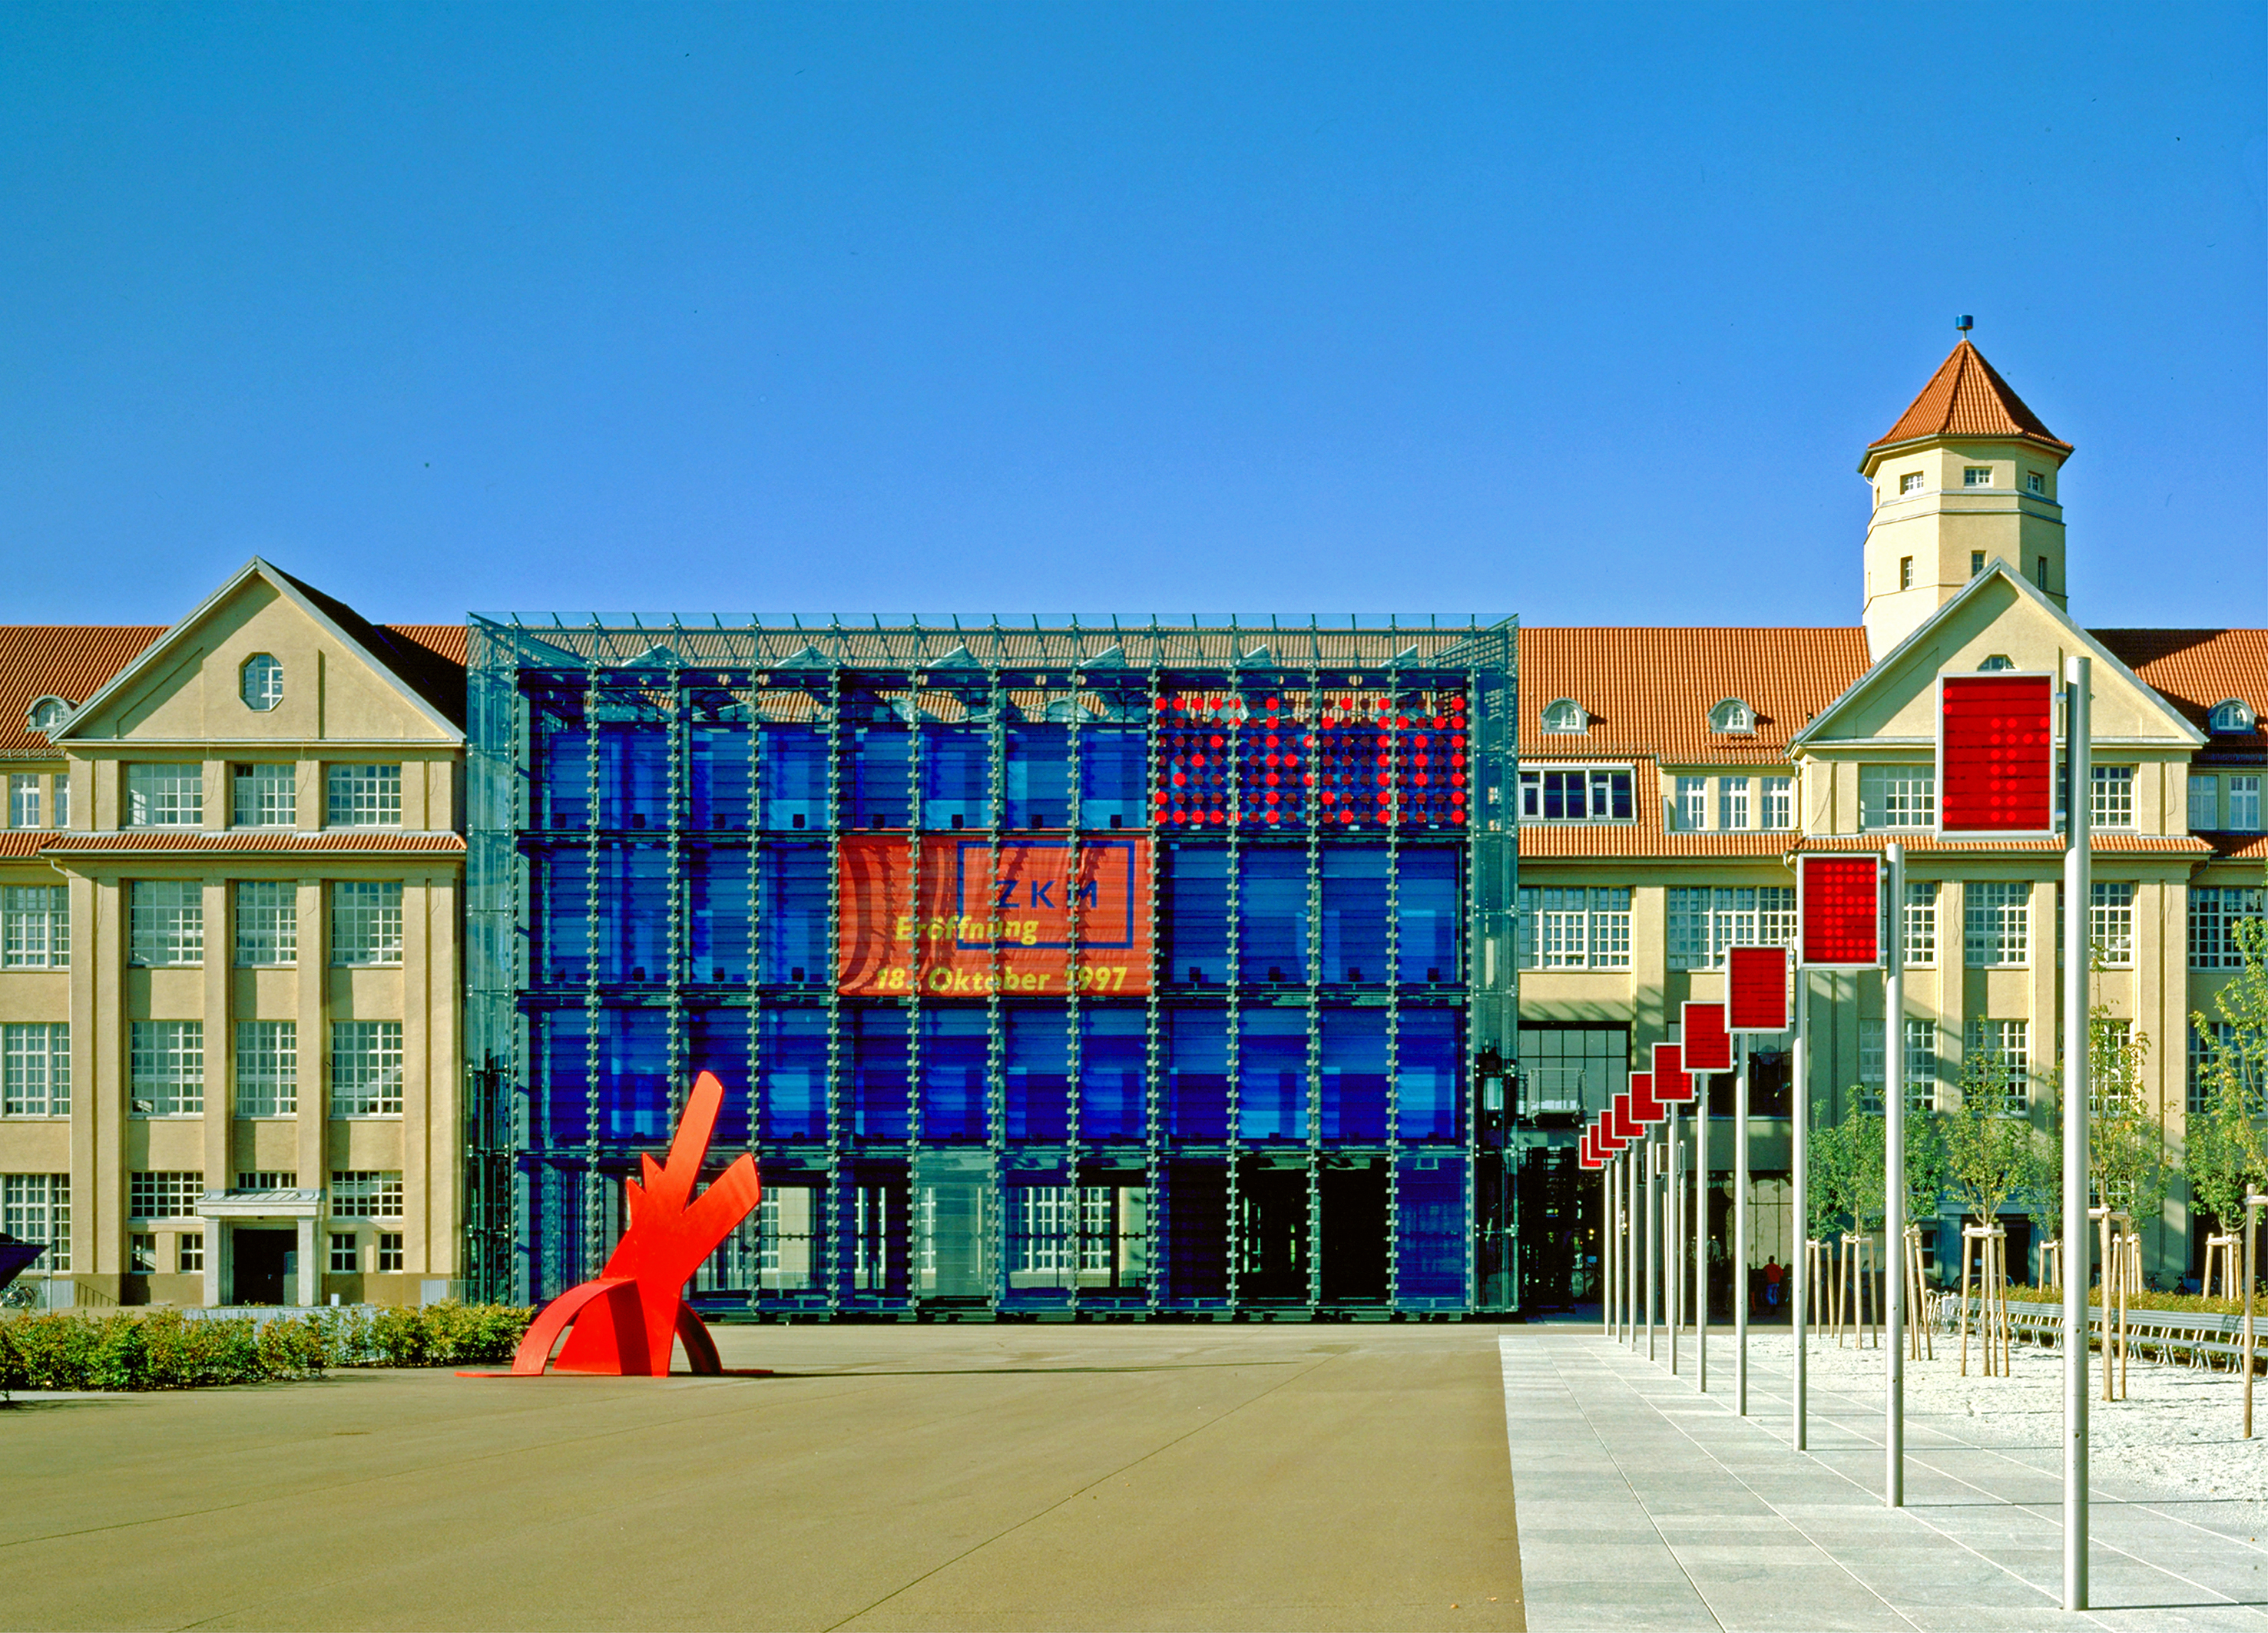
\includegraphics[width=0.7\textwidth]{img/zkm-commons.jpg} 
%\captionsetup{justification=centering}
\caption{ZKM - wikimedia commons}
\end{figure}

\textit{Sveti Kliment} (2007) by Robert Sazdov and was recorded at the Sonic Lab of the Sonic Arts Research Centre (SARC) in Belfast, Northern Ireland. The composition was inspired by Saint Clement of Ohrid from the Orthodox Church of Macedonia, a patron saint of education and language who committed his life to: research, teaching, and improving the lives of "those in his diocese". The piece open with the natural sound of a flute but quickly morphs into a soundscape of reversed noises and unintelligible speech snippets. The timbre of the flute reappears as a thematic motif and its reverberation is frozen and played over, using the same instrument. The timbre of the flute seems to be that of a ethnic instrument perhaps in reference to the Balkans. 

\textit{Morphons and Bions} (2011) is a real-time Puredata composition which relies on noise synthesis and randomness. \cite{hagan2012aesthetic} provides a richer description of the work. As opposed to Sazdov's piece, all the sounds in this piece are synthesized in real-time. According to Hagan: 

\begin{quote}
    "Because the work is built on a substrate entirely made of noise, the piece is situated within certain philosophical and aesthetic issues surrounding noise, its use, and its definition."
\end{quote}

Indeed, a lot of discussion has gone into the role of noise in contemporary music. Despite the abundance of noise in \textit{Morphons and Bions}, Hagan does not consider the piece to fall under the category of "noise music", given the harmonic and quasiharmonic patterns that emerge from the organization of sounds. One interesting ontological point raised by Hagan is the idea of noise being the main source of information in this work. This goes against established notions of engineers seeking to remove noise from signals. As she says: "the noise \textit{is} the signal". 

\cite{hagan2017textural} provides more technical information on the piece. Here, Hagan describes the two main synthesis method employed by this work, which were later combined into one. The first she describes as additive synthesis modulated with white noise which results in the following equation:

$$
x(t)=\sum_{k=1}^{6} w(t) \sin \left(2 \pi h(t) f_{0}(t) t+D(t) n(t)\right)
$$
where \\
$n(t)=$ white noise, \\
$D(t)=$ depth (amplitude of white noise) changing in time, \\ 
$f_{0}(t)=$ fundamental frequency changing in time, \\
$k=$ partial number, \\
$w(t)=$ Gaussian random variable with mean $1 / k$, and \\
$h(t)=$ Gaussian random variable with mean $k$.\\

As you can see the equation shows both AM and FM with noise as the modulating signal. Hagan also describes the use of band-pass filters with aleatory properties to further articulate her sounds. Hagan has adopted the terms "textural composition" to describe her music. Her work in this domain draws from the philosophical frameworks of Russolo, Cage, and Xenakis, and is driven by statistical methods, such a Gaussian distributions. \href{http://www.kerrylhagan.net/#m&b}{Her site} contains all the associated patches required to perform the piece live. Given the aleatory nature of the work, each rendition should be subtly different.

\textit{Il Prete Rosso} (2013) Charles Nichols is a work for amplified violin, motion sensor and computer, written for Sarah Plum. The piece was inspired by Antonio Vivaldi, teacher and violin virtuoso, and translates to "The Red Priest" - nickname given to Vivaldi for his red hair and ordinance. In the piece the violin is looped live and played over while recorded elements are spatialized. The computer musician interjects with a wah filter, phaser and delay effects. The motion sensor, attached to the violin player is used to control the center frequency of the wah filter. The work was premiered at the Cube of the Moss Arts Center at Virgia Tech which yields an impressive 124.4 channel system.

The fifth piece in this anthology titled \textit{He Slowly Fell, and Transformed into the Terrain} (2016) was composed by Natasha Barrett in sixth-order Ambisonics using IRCAM's Spat software. This piece is the longest from the collection lasting over 20 minutes. The composer applies HOA granular synthesis, a technique in which sounds are fragmented into thousands of smaller units for re-synthesis, applied to soundfield recordings captured using a FOA commercial microphone. An interesting aspect of the work, not mentioned in the text, is the concept of privacy. Audio recordings taken in public are problematic as source material. Certain laws exist prohibiting artists to use these materials without permission. Through the use of granular synthesis, the material quality of voices is maintained, but the dialogue because unintelligible, making this a non-issue. \cite{barrett2016musical} also references the HOA granular synthesis unit developed at IRCAM. The system, titled \textit{Grandad} encodes each individual grain of sound in 9th-order ambisonic and can be heard in the second movement of \textit{Hidden Values} (2012), also by Barrett. 

\textit{Space, S[acred|ecular]} (2015) was written by Fernando Lopez-Lezcano using impulse responses capture at Hagia Sophia: a cathedral turned mosque turned museum, featuring a reverberation time of over ten second\footnote{Depending on where the impulse response is taken.}. The building in Istanbul, Turkey, was acoustically sampled in order to recreate its sound using a new reverb technique for Higher Order Ambisonics (HOA). Fernando's use of two instruments, voice and percussion, alludes to the dual nature of the religious space.  \cite{lopez2014architecture} describes the reverb method, which consists of using an intermediary decoder for the convolution reverb. This means that the HOA reverb can be implemented even if the playback system does not support HOA. The impulse responses were processed from balloon pops using an analysis/re-synthesis method which measures echo density and energy at multiple frequency bands. The technique was informally compared in a listening test with the favoured sine swept technique to good effect \cite{abel2010estimating}. The entire piece was written in \href{https://ccrma.stanford.edu/software/snd/snd/s7.html#juce}{s7}, "a Scheme implementation [of Common Lisp Music] intended as an extension language for other applications\footnote{Scheme is a programming language which is part of the Lisp family. Lisp is one of the oldest low-level programming languages (only Fortran is older by one year).}". The mixing process, as well as the reverb, were all implemented using open source software. This included the binaural decoding which suggests that, in theory, no HDLA is needed for creating music for these systems. 

\begin{figure}[ht!]%force figure here, top, strict
\centering
\includegraphics[width=0.7\textwidth]{img/hagia-sofia.jpg} 
%\captionsetup{justification=centering}
\caption{Hagia Sofia - wikimedia commons}
\end{figure}


The final piece discussed included in the anthology comes from Gerriet K. Sharma and is titled \textit{mirage 4} (2015). The piece was composed with and for the icosahedral\footnote{Speaker approximating a sphere with 20 faces and one speaker for each phase of the geometry.} loudspeaker developed by the Institute of Electronic Music and Acoustics (IEM) at the aforementioned ZKM\footnote{ZKM stands for "Zentrum für Kunst und Medien" which translates to "Center for Art and Media Karlsruhe", Karlsruhe the city in Germany where the cultural center is located.}. This icosahedral speaker, takes the concept of ambisonic microphones, which capture soundfields at a single point, and invert the mechanism, attempting to project a soundfield from a single point in space, with increasing resolution based on the number of transducers. 

\cite{wendt2017perception} by Wendt, Sharma, et al. discusses the ability of such a system to reproduce accurate spatial dimensions of sound for compositional means. The system is indeed capable of creating the impression of moving trajectories of sound by exploiting wall reflections which are perceived as virtual sources. These coincident speaker arrays can be considered as a portable and affordable means for spatial music reproduction. The greatest benefit these provide, for composers, is the ability to reproduce \textit{periphonic} spatial music, that is, sound with height, without having to rely on the venues' loudspeaker array. 

Ontologically, Sharma has framed his composition using the language of sculptors, discussing at length about materiality of sound, and the treatment of space as a plastic - and malleable - medium. Unfortunately, the recording included seems to suffer from significant noises, which I don't believe were intentional. These were picked up by the binaural recording system during the recording of the piece. It is however, entirely possible that these sounds \textit{are} intentional. The predominant sounds in the work are long, noisy, and soft. The piece reminds one of an ethereal, nebulous cloud, floating above them. There is a clear motif, with identical pitches reappearing at different points of the piece together with synthesized drones. 

\subsection{Installation works}
%https://escholarship.org/content/qt4d50k2fp/qt4d50k2fp.pdf

\subsection{Video games}
%  http://www.visual-memory.co.uk/b_resources/Munday%202007%20Music%20In%20Video%20Games.pdf

\subsection{XR Experiences}
% https://dl.acm.org/doi/pdf/10.1145/3359997.3365740?casa_token=En3ZeasOIT4AAAAA:pCmykPbrMvlNNHmyiiBzEhRScdcc1JyXM9R9Pl20Jsa-_rR6fMnWJIj33W0MMDZHPHrvXpR5PA

\section{Open tools for spatial music}\label{sec:open_tools_spat_mus}

This section will provide an overview of different existing tools for computer musicians which facilitate the creation of spatial music. We will focus on free and open source tools which work inn conjunction with computer music languages such as Pd, SuperCollider, Csound, etc. 

 

\section{History of Spatial Instruments} \label{sec:spat_instruments}
%older
\section{Contemporary Spatial Instruments}

This section will discuss the development of \textit{spatial instruments} in the 21st century. The term \textit{spatial instrument} refers to instruments which allow the user to manipulate spatial elements of sound. Spatial elements might include: direction, reverberance, width, etc. Traditional instruments generally allow the performer control over dynamics, pitch, and sometimes timbre. In contrast, \textit{spatial instrument} give the performer augmented control by allowing the user to modify the position of sound in space, whether that be for multi-channel sound reproduction or binaural synthesis\footnote{Virtual surround sound over headphones.}. 
Many instruments of this nature have been developed over the last few decades due to the popularity of multi-channel reproduction in electro-acoustic music. The development of such instruments goes back to the 1950s in fact, with pioneering works by composers such as Pierre Schaeffer. In contrast to our common definition of instruments, many of the interfaces which will be described in this section do not produce sound at all. In fact, much of the development in Human Computer Interaction (HCI) related to this field has focused solely on the manipulation of sound in space as separate practice from mapping controls to sound synthesis methods.  

\cite{pysiewicz2017instruments} presented a comprehensive ethnomusicological review of \textit{spatial instruments}. In that reference, the authors described a \textit{taxonomy} for the different types of spatial instruments. The three main categories from the 31 different spatialization interfaces found were: acoustic instruments extended to allow for spatial control, interfaces for the manipulation of spatial elements of sound only, and interfaces both for manipulation of spatial elements of sound as well as synthesis parameters. 

In the following sections we will describe some of the instruments created by pioneering composers from the early days of electro-acoustic music, as well as contemporary inventions which could lead to new compositional approaches. Our motivation is to understand the state-of-the-art and consider approaches which have not previously been undertaken. As we explore these different instruments we will expound upon their viability for an open-source approach to spatial music. 

\subsection{Controllers}
\subsection{Augmented instruments}
\subsection{Real-time spatial synthesis}

\section{Open Tools for Spatial Instruments}

\section{The Future of Spatial Music \& Instruments}

\section{Conclusion}



 
%spatial audio (fixed-media) [REC/REPRODUCTION]
\chapter{Spatial Audio: Capture \& Reproduction}

\todo[inline]{I am not sure but I think this chapter is too long. I might need to split it into capture for one chapter and reproduction for another chapter. I can also just put reproduction into chapter 2. It might be ok.}

\section{Introduction}

This chapter will be developed with Tamara Smyth. In this chapter, we will shift the focus from spatial music to spatial audio. We will begin by drawing a line from the inception of recorded sound to the latest developments in 3D audio, including advancements in cross-talk cancellation (XTC), WFS, and ambisonics. In this chapter, we are concerned with the variety of ways that sound engineers can use spatial audio technologies to record and reproduce spatial music: whether that be in real-time or asynchronously. We will also touch upon some of the technical complications of this work that might prove problematic for engineers (ie. insufficient memory, speaker count, hardware requirements, etc.).

In particular, this chapter will focus on the main technology this author is concerned with: ambisonics. One of the major benefits of ambisonics is the \textit{isotropic}\footnote{Identical in all directions; invariant concerning direction. In an ambisonic context, this means the sound field can be reproduced in whatever sound system is available.} nature of the design, which makes it more flexible than surround sound standards such as 5.1. Ambisonics has a long-established tradition in the spatial audio community and as such, a myriad of open source tools have already been developed for its usage. These tools make it more accessible in many ways that \textit{object-based audio} (OBA) ecosystems. With the proliferation of systems for binaural rendering, ambisonics has resurfaced as a reliable method for spatial audio reproduction.

In addition to listing and demystifying the different spatial audio technologies available today for playback, we will suggest engineering approaches for the capture of spatial sound both for real-time transmission and for asynchronous dissemination using open-source technologies. We will focus on spatial audio recording techniques and describe systems based on freely available software for mixing and mastering spatial audio which can later be used in immersive environments such as the ones described in Chapter \ref{ch:xr-mus}. In contrast to Chapter \ref{ch:spat-mus}, which outlines technologies which are better suited for real-time performances with musicians, in this chapter we will focus more on tools for creating \textit{fixed-media} works.

\section{History of Spatial Audio Capture}

In the previous section of this paper we presented a number of composers who made space an integral part of their practice as well as \textit{spatial instruments} used for the development of such works. This next section will describe the development of modern spatial audio systems from an historical and engineering perspective. 

% Many engineers must be thanked for giving composers the ability to \textit{diffuse} sound in space towards musical ends. In this section we will discuss some of the most influential engineers that have contributed to the development modern \textit{spatial audio} systems. 

% The chapter will be divided into four sections: 

% \begin{enumerate}
%     \item Spatial audio developments before the 21st century
%     \item Contemporary spatial audio developments in sound recording
%     \item Contemporary spatial audio developments in sound reproduction
%     \item Overview of open tools for recording and playback of spatial sound
% \end{enumerate} 

\subsection{Audio Pioneers} \label{subsec:audio_pioneers}

The invention of the telephone, in 1876, by  Alexander Graham Bell \cite{grosvenor2016alexander}) can be considered the genesis of all \textit{spatial audio} technologies. The transmission principles it used where what later inspired the development of the phonograph, one of the first known recording devices, invented by Thomas Edison in 1877 \cite{gitelman1999scripts}, and, subsequently, galvanized a whole new generation of engineers who developed more sophisticated methods for sound capture and reproduction. 

\begin{figure}[ht]%force figure here, top, 
\centering
\includegraphics[width=0.7\textwidth]{img/theatrophone.jpeg} 
%\captionsetup{justification=centering}
\label{fig:theatrophone}
\caption{Théâtrophone \cite{theatrophone_pic}}
\end{figure}

A few years after the invention of recorded sound, Clement Ader, best known for his work in  aviation, would present the \textit{théâtrophone}, a "system of telephonic transmission where listeners received a separate channel for each ear, enabling stereophonic perception of actors on a set" during opera performances. Just a year before, Ader had presented his prototype at the Paris Exhibition for Electricity in 1881 \cite{malham19953}. Figure  \ref{fig:theatrophone} shows a picture of the device. We can see the two receivers which would be placed at the listeners ears for \textit{stereophonic} audition. The writing on the image also shows the cost for the audience member, which was 10 minutes for one franc, or 5 minutes, for 50 cents. 

Decades would pass before any new major developments in the field would occur, but eventually, in the 1920's, Harvey Fletcher, from Bell Telephone Laboratories\footnote{Bell labs has an important place in computer music history. It is where Max Mathews wrote the first computer music language, MUSIC-N.}, developed one of the first binaural recording systems. This system used the anatomy of the head to naturally embed spatial attributes of sound to recordings \cite{harvey1927binaural}. It would not be, however, until 1933, at the Chicago Century of Progress Exhibition, that binaural recordings would first be introduced to the public. 

Fletcher is believed to also be responsible for the first public demonstration of stereophonic sound, which took place in 1934 in New York City. Bell Telephone Laboratories, along with Fletcher, is also accredited for, in the 20's, being the first American institutions to research what is known today as wave-field synthesis (WFS): a system which captures a "wall of sound", using an array of microphones, and then consequently plays it back, using an array of speakers. In other words, engineers would mount a curtain of microphones and then reproduce the recorded signals using a curtain of speakers of similar proportions\cite{fletcher1942hearing}\footnote{While Fletcher would be one of the first to describe the idea of WFS in 1942, it would not be until 1988 that Berkhout would propose the mathematics involved in WFS to transform a single sound source into a wall of sound.}.

Later, in 1933, Fletcher also demonstrated the possibilities of long-distance multi-channel sound transmission. In a collaboration with English conductor Leopold Stokowski, considered one of the first stereo control-board operators\cite{mcginn1983stokowski}, Harvey and other Bell Lab engineers put together a system which transmitted the sound of an orchestra in Philadelphia via three microphones placed on stage to three corresponding loudspeakers in Washington DC's Constitution Hall. Bell Labs and Stokowski would go on to collaborate on numerous events in the 40's. Around the same time Alan Blumlein, an American engineer, was working on a much simpler yet powerful spatial audio technique: high-fidelity stereophony. 

Blumlein's most important contribution to the field of spatial audio is perhaps his mid-side (MS) encoding technique, patented in 1931 \cite{billingsley1987simulated}. This technique allowed audio engineers to mix stereo and mono information,  towards spread control, by summing and subtracting signals with equal and inverted phase. The technique was later expanded by Gerzon to develop a First Order Ambisonic\footnote{Also known as tetrahedral microphone} microphone. The idea consisted of taking the output of a \textit{figure-8} microphone and summing it with an \textit{omni-directional} microphone. A second copy of the figure-8 microphone would be phase inverted. The result were two cardioid like patterns with the same orientation as the stereo-speaker arrangement. Figure \ref{fig:ms_stereo} shows the general set-up for the MS stereo recording technique, note the panning on the two copies of the figure-8 microphone. 

\begin{figure}[h!]%force figure here, top, strict
\centering
\includegraphics[width=0.35\textwidth]{img/ms_stereo.svg.png} 
%\captionsetup{justification=centering}
\label{fig:ms_stereo}
\caption{Mid-Side Stereo \cite{ms_stereo_pic}}
\end{figure}

One of the biggest moments for spatial audio occurred at the very end of the decade. In 1940, Leopold Stokowski, RCA, and Disney would release the film \textit{Fantasia} which featured a system called \textit{Fantasound}. The control system they designed allowed audio tracks to be panned to any of 10 loudspeakers \cite{klapholz1991fantasia}. This lead to an era of development in professional theatre systems with much to be desired on the consumer end. Moderate improvements to sound quality and storage capacity were achieved from 1940 to 1970.

In the 1970's, a new and significantly more obscure technology began being developed: \textit{quadraphonic sound}. Quadraphonic research is believed to have begun at the Acoustic Research Corporation by Robert Berkovitz \cite{davis2003history}. The idea was to use two rear channels commercially to produce the ambience of the recording and two front channels for direct sound. Unfortunately, due to a number of financial, engineering, and marketing issues, the system never gained much popularity. Fortunately, the system did inspire other developments. 

The development of encoding and decoding schemes for quadraphonic sound would eventually peak the interest of British mathematician Michael Gerzon. Michael would, in 1969, present to the public a new audio capture method inspired by Alan Blumlein and the rise of interest in quadraphonics. Gerzon proposed, provocatively, the use of a tetrahedral array for audio capture in which the four signals could be encoded into three coincident\footnote{Coincident here meaning placed close together.} figure-8 microphones. This system, Gerzon believed, could optimize the use of the four speakers by providing listeners with not only horizontal information, but also vertical sound. Unfortunately, the system suffered from a considerably small ideal listening area\footnote{Also called \textit{sweet spot}. Higher Order Ambisonics (HOA) has been shown to increase the size of the sweet spot.}, a fact which detracted sound system engineers who were primarily concerned with audio for film, as it had become, and possibly remains, the focus of spatial audio research. 

Around the same time, in 1970, Tom Horall of what today is known as Acentech\footnote{https://www.acentech.com/} decided to attempt to recreate the acoustics of the famous Boston Symphony Hall using a acoustic model approximation. The system used tape delay techniques to achieve believable spatial sound. Using a dozen loudspeakers Horall was able to convince the listeners that they were actually being transported to the iconic hall. The system would later be commercialized in 1988 and become known as the Pioneer DSP-3000 \cite{davis2003history}. 

Many other developments followed suit from the 80's to today. Perhaps the most popular of these is 5.1 surround sound, a popular audio system which has had decent success commercially. Today, there is an ongoing battle regarding the future of spatial audio. Companies are consistently looking for scalable and reliable solutions to improve sound quality for patrons. Unfortunately, many of these systems have suffered from their distinctly complicated set-up process or high costs. The quest for: simple, high-fidelity, three-dimensional sound; is one that will, likely, not end soon. 

%\subsection{Stereo Techniques}
\subsection{Binaural Microphones}

\textit{Binaural audio} and \textit{multi-channel stereophony} are the two most common spatial audio technologies. \textit{Binaural audio} has become increasingly popular for \textit{virtual reality} (VR) while \textit{multi-channel stereophony} can be found in home entertainment systems as well as automotive sound systems. Stereo, however, is still the prevailing reproduction format, which is why binaural microphones have gotten some interest as a means of "static" spatial audio reproduction. Others have written about \textit{transaural} sound systems, which reproduce \textit{binaural audio} over stereo systems. \textit{Transaural} reproduction is a niche system that has been gaining more interest in the community. The underlying technology, however, seems to remain limited to audiophiles and a number of select engineers working on it.

In contrast to other spatial audio recording methods which rely on large arrays of microphones binaural recordings only use two microphones to encode spatial information into a stereo recording. Binaural recordings are either captured using a \textit{dummy-head}, a mannequin head with microphones inside its ears, or with \textit{in-ear} microphones placed inside a person's ear canals, to capture what they would normally listen to. By playing back these binaural recordings using headphones, ear-buds, or with stereo speakers using \textit{cross-talk cancellation} (XTC) filters\footnote{XTC is also referred to as \textit{transaural reproduction} in the literature.}, a person can sense a sonic space around them as it originally occurred. 

Unfortunately, some issues arise from this method. Firstly, people's heads and ears differ in size and shape, a fact which distorts the recordings ever so slightly breaking the illusion that one has been transported from their current location to the new auditory scene. Secondly, when the listener hears back the recording, they will be striped of rotational control. In other words, when they turn their heads, the sound will remain fixed in the same perspective as the original recording, and the illusion of immersion will be lost. This lack of \textit{auditory parallax} creates localization errors and \textit{internalization} of sound sources. Figure \ref{fig:dummy-head} shows a "dummy head" - a binaural microphone with two capsules placed inside the modeled pinnae, mimicking the behavior of the human cochlea\footnote{The biological structure in our inner ear where frequency analysis is performed.}. The \textit{pinnae} in these systems tends to be manufactured using a soft plastic such as silicone to mimic the absorption of human cartilage on sound.

\begin{figure}[ht!]%force figure here, top, strict
\centering
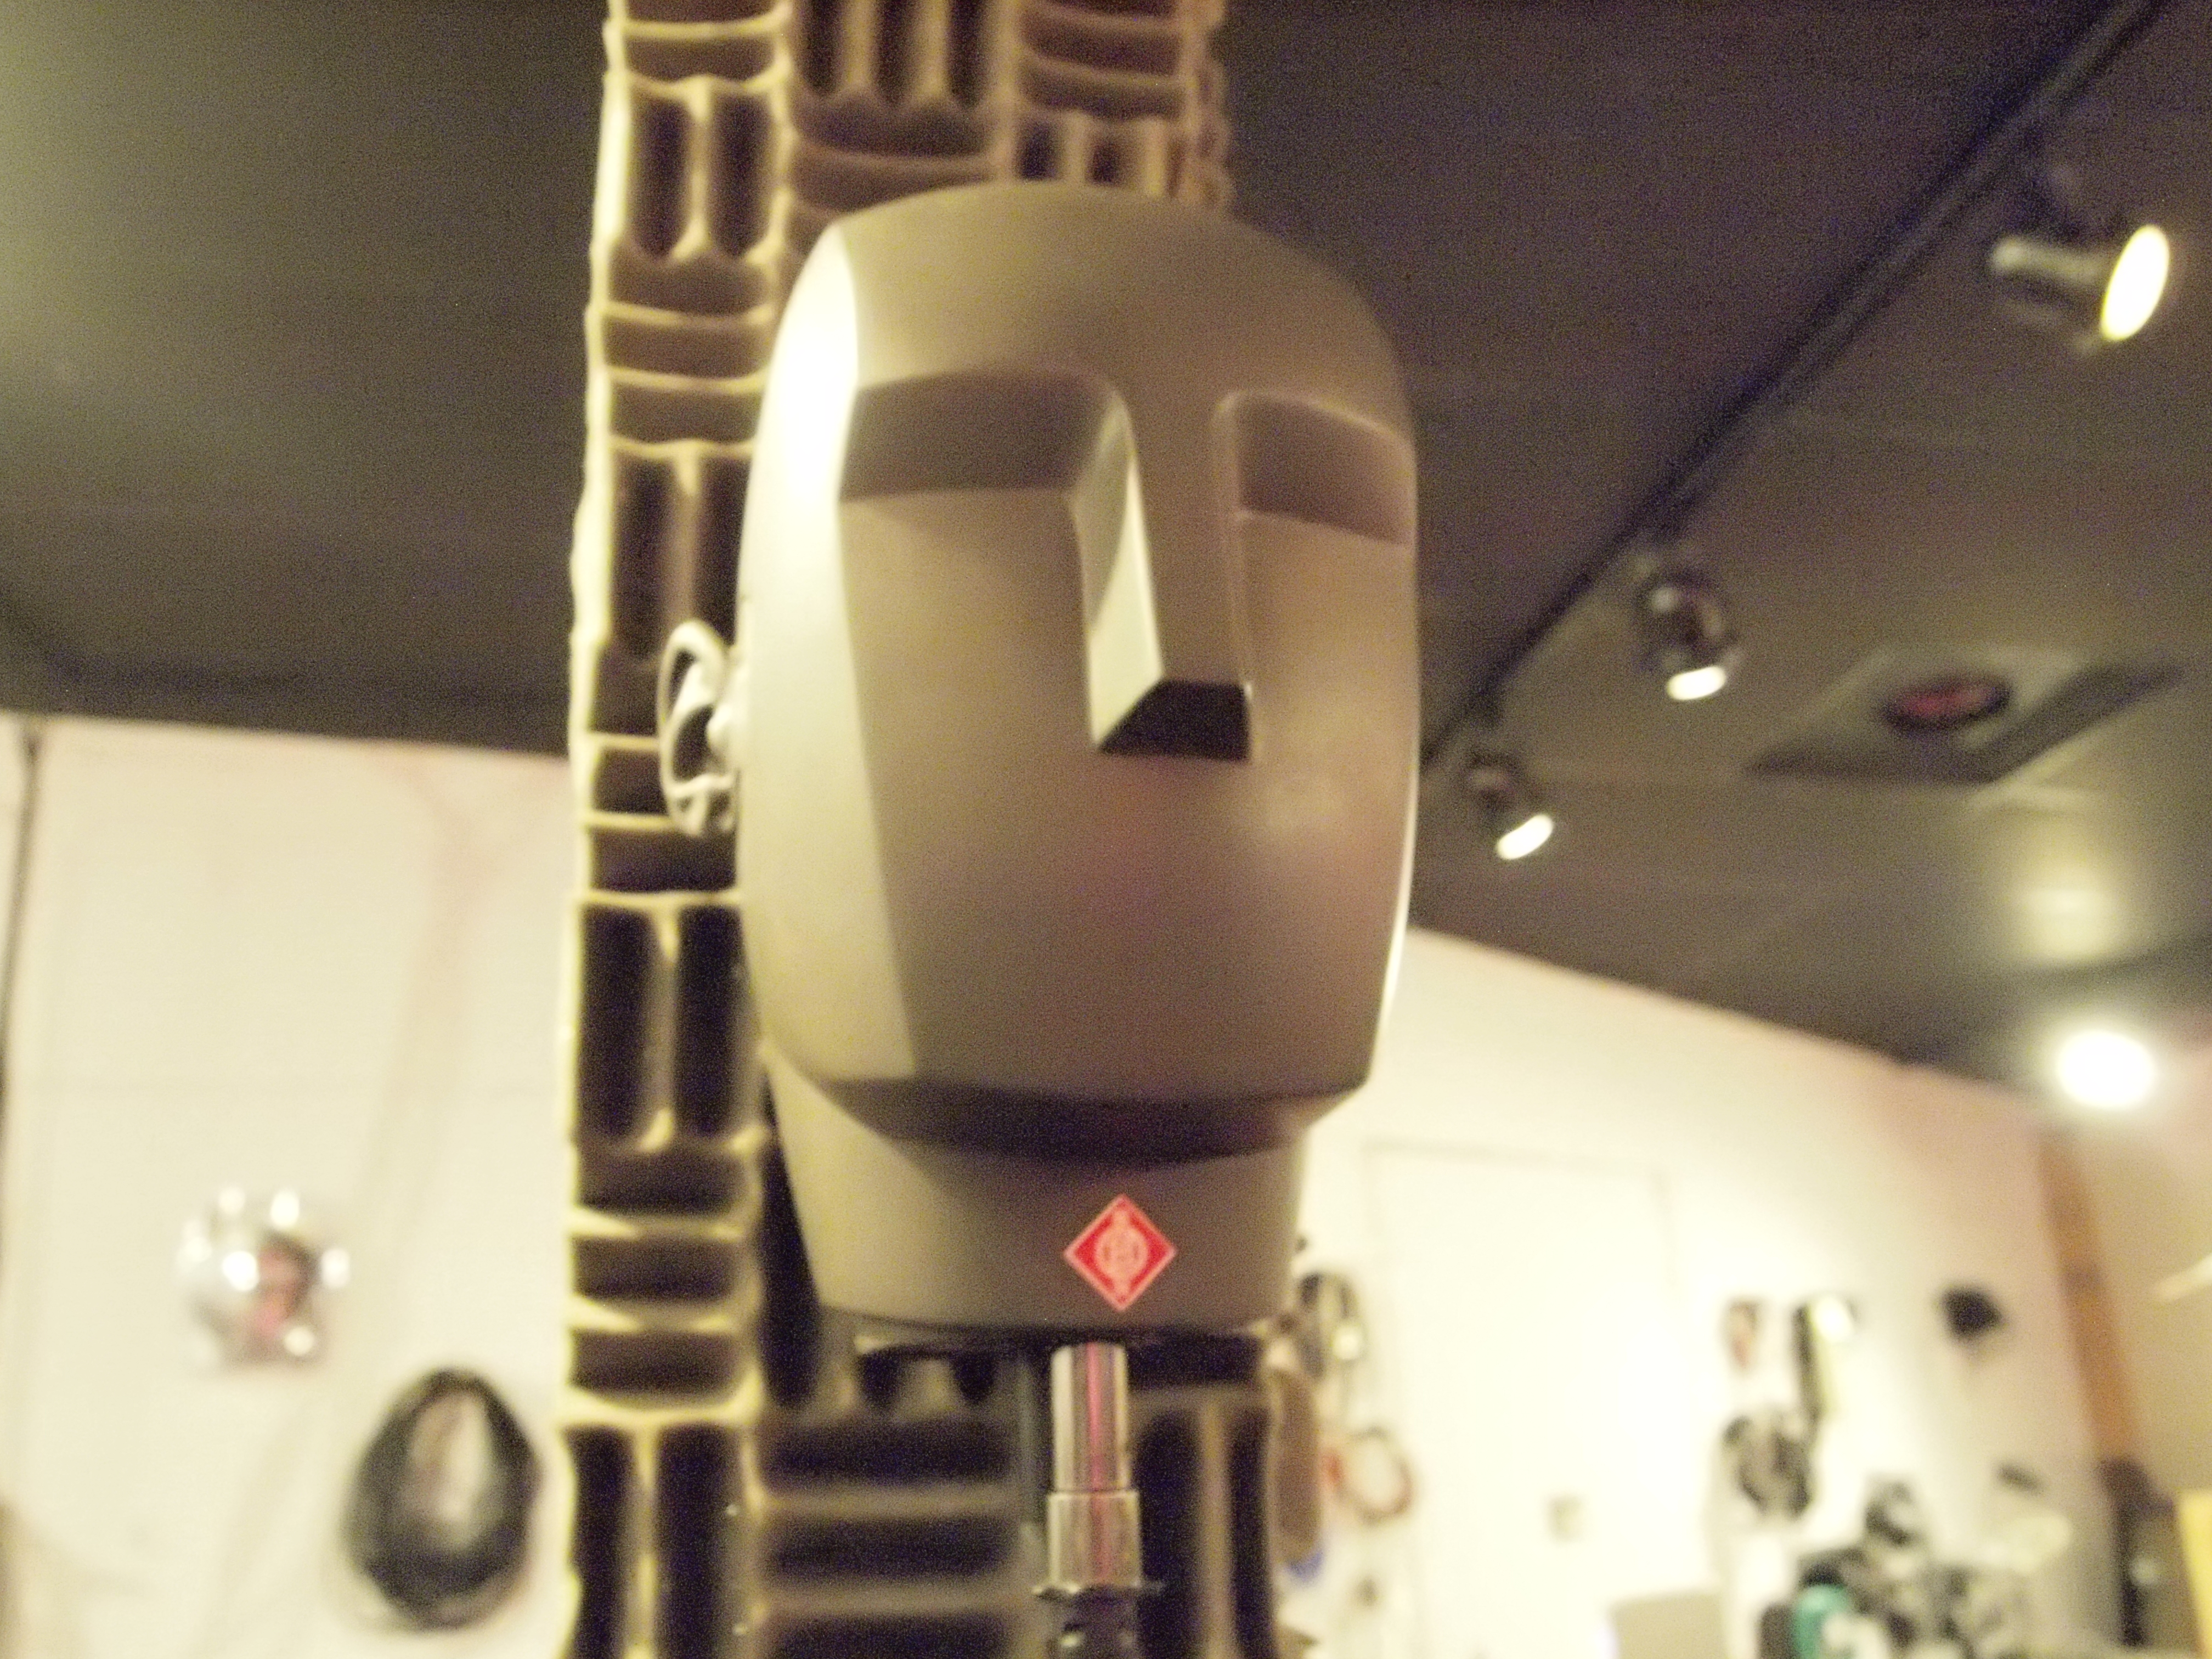
\includegraphics[width=0.7\textwidth]{img/dummy-head.jpg} 
%\captionsetup{justification=centering}
\label{fig:dummy-head}
\caption{Dummy Head - wikimedia commons}
\end{figure}

\textit{Binaural recordings} are not a particularly good representation of the desired soundfield resulting from a \textit{spatial music} work, however, they are crucial for the development of binaural synthesis systems, which ultimately can convey a proper representation of the musical work. Often, it becomes impractical to use a real human for HRTF sampling since the process can take quite a long time and human movements during acoustic sampling can lead to errors in the dataset. In this context, an anthropomorphic average of a human is better suited for the sampling task. Alternatively, the binaural impulse responses can be synthesized using acoustic models. \cite{algazi2002use}, for example, describes a head-and-torse model, or "snowman" model, to efficiently implement HRTF approximations towards real-time spatialization. 

\begin{equation} \label{eq:conv-hrir}
\begin{array}{l}
x_{L}(n)=\sum_{p=1}^{P} x_{p}(n) * h_{L, \theta_{p}, \phi_{p}}(n) \\
x_{R}(n)=\sum_{p=1}^{P} x_{p}(n) * h_{R, \theta_{p}, \phi_{p}}(n)
\end{array}
\end{equation}

\cite{hacihabiboglu2017perceptual} provides a simple equation for the \textit{auralization} of a virtual signal via convolution with two HRIRs. This is equivalent to the process of filtering the source $x_p$ with a filter whose frequency response would be identical to the Fast Fourier Transform (FFT) of $h_{R, \theta_{p}, \phi_{p}}$ and $h_{L, \theta_{p}, \phi_{p}}$ respectively. The topic of \textit{binaural synthesis} will be further discussed in later sections, as it is a primary topic of this work, which warrants extensive discussion.

\subsection{Soundfield microphones}

History of soundfield microphones.

\section{Contemporary Spatial Audio Capture Techniques} \label{sec:contemp_audio_capture}

While the popularity of spatial music has become evident in the electro-acoustic domain, little effort seems to have been devoted by composers for the accurate representation of their music in a recorded format. Often, composers opt to use stereo recordings of their work, due to the complexity of spatial audio recording technologies or their lack of availability. While in previous sections of this work we have focused on technologies which allow the creation of spatial music, in this section we will focus on hardware and software which allows one to document their works, with differing degrees spatial quality retained, for public dissemination outside of the concert hall. 

\subsection{Multi-channel Spaced Microphone Arrays}
%https://www.dpamicrophones.com/mic-university/immersive-sound-object-based-audio-and-microphones

Before we can begin to understand contemporary 3D audio capture techniques we should discuss some fundamental microphone principles. All spaced microphone arrays rely on systems which turn air pressure changes into electrical currents and subsequently binary information, which represent these pressure changes as sampled in time. Most well-known \textit{monophonic} microphone types fall within the family of cardioids. The general equation for the family of cardioids is:

\begin{equation}
    \rho(\theta) = \alpha + (1-\alpha)cos(\theta)
\end{equation}

This equation, from \cite{ortolani2015introduction}, provides a way for us to construct the most common types of \textit{polar patterns} found in commercial microphones today. \textit{Polar patterns} depict the sensitivity of a microphone to sound pressure as a function of the direction-of-arrival (DOA) and are frequency dependent. The most important patterns for our purposes are: \textit{omni-directional} where $\alpha=1$ \textit{cardioid} where $\alpha = 0.5$, and \textit{figure-of-eight} where $\alpha=0$. Figures \ref{fig:card}, \ref{fig:omni}, and \ref{fig:fig-8} show the polar patterns of these three popular types of microphones. 

\begin{figure}[!htb]
\minipage{0.32\textwidth}
  \includegraphics[width=\linewidth]{img/card.png}
  \caption{Cardioid Polar Pattern \cite{card_pic}}\label{fig:card}
\endminipage\hfill
\minipage{0.32\textwidth}
  \includegraphics[width=\linewidth]{img/fig-8.png}
  \caption{Figure-8 Polar Pattern \cite{fig8_pic}}\label{fig:fig-8}
\endminipage\hfill
\minipage{0.32\textwidth}%
  \includegraphics[width=\linewidth]{img/omni.png}
  \caption{Omni Polar Pattern \cite{omni_pic}}\label{fig:omni}
\endminipage
\end{figure}

These idealized responses show the sensitivity of different microphones to sound waves arriving from different directions. For the cardioid\footnote{Which gets it's name from it's heart-shaped response.} pattern, we see a \textit{null} at 180\textdegree and \textit{unity} response at 0\textdegree. These diagrams are seldom true in real-life, especially for high frequencies. Even for very good omni-directional microphones, eventually the capsule size becomes comparable to that of the wavelength, making the response directional. 

\textit{Off-axis coloration} refers to microphone's difference in frequency response at different directions. Most microphones can intuitively be separated into \textit{side address} or \textit{front address} microphones based on their construction. For \textit{front address} microphones, the reported frequency response will likely be based on a measurement with the capsule facing the excitation source so the response matches the ergonomic use of the microphone. Any \textit{side address} microphone, such as a cardioid condenser microphone, would perform poorly if the musician oriented the microphone backwards, resulting in a different frequency response than expected.

\textit{Proximity effect} is another term which relates to the nature of unidirectional microphones\footnote{Cardioids and figure-8 microphones fall under this category.} to exhibit a bass-boost when placed too close to the source. This is why many condenser microphones come equipped with a bass roll-off switch. The bass-boost comes from the \textit{pressure gradient} microphone. At low enough frequencies, the wavelength is vastly larger than the microphone capsule, so the difference in pressure at either side can be unnaturally large. This effect should be considered when placing musicians in relation to the microphones.

The mid-side (MS) technique previously discussed is just one of several stereo techniques that are traditionally implemented for stereo recording. While other stereo techniques such as A/B, X/Y, and ORTF also exist, these fall outside the scope of this text. The reader is referred to \cite{lipshitz1986stereo} for a lively discussion on the merits of coincident and spaced arrays for stereo reproduction. It warrants mentioning that by no means are surround-sound techniques objectively superior. In fact, there is still a lot of research being undertaken in this domain, in particular by The University of Huddersfield \cite{lee3d}. 

\textit{Spaced arrays} are a family of microphone arrays designed originally for surround sound formats. Various authors over the years have experimented and documented their configurations in order to facilitate the creation of high-quality multi-channel music for film. Figure \ref{fig:c-spaced-arrays} shows five complete spaced arrays adapted from \cite{hacihabiboglu2017perceptual} and \cite{politis2016microphone}. The diagram created is a rough approximation of these five 5.1 arrays. In addition to these five arrays, ambisonic arrays are also considered complete \textit{coincident} arrays capable of encoding surround sound formats. \cite{Immersiv9:online} also provides information about these arrays\footnote{Distances and angles might be slightly different from one reference to another. \textbf{TODO}}.

% 5.1 arrays (Fukada Tree, INA-5, Hamasaki Tree, DPA 5100, OCT-surround)
\begin{figure}[ht!]%force figure here, top, strict
\centering
\includegraphics[width=1.0\textwidth]{img/complete-spaced-arrays.jpeg} 
%\captionsetup{justification=centering}
\label{fig:c-spaced-arrays}
\caption{Complete Spaced Arrays}
\end{figure}

\todo[inline]{The symbols I used for these drawings are not standard. Not sure if that is ok.}

In addition to the five depicted arrays:
\begin{enumerate}
    \item \textbf{Fukada Tree}
    \item \textbf{INA-5} 
    \item \textbf{Hamasaki Tree}
    \item \textbf{DPA 5100}
    \item \textbf{OCT-surround}
\end{enumerate}

% Front arrays (Optimal Cardioid Triangle, Decca Tree, INA-3). Rear arrays (Hamasaki Square, IRT Cross)

A secondary technique exists for multi-channel audio recordings which involves a combination of a proximal front array and a distant rear array. In this configuration it is up to the sound engineer to decide how distantly the rear array will be placed. The decision will be based generally on the size of the space as well as how diffuse the sound is at the set distance. Front arrays include: Optimal Cardioid Triangle, Decca Tree, and INA-3. Rear arrays include: Hamasaki Square, and IRT Cross. Figure \ref{fig:fnr-arrays} shows a coarse approximation the associated arrays.

\begin{figure}[ht!]%force figure here, top, strict
\centering
\includegraphics[width=1.0\textwidth]{img/front-n-rear-arrays.pdf} 
%\captionsetup{justification=centering}
\label{fig:fnr-arrays}
\caption{Front and Rear Arrays}
\end{figure}

\subsection{Encoding Monophonic Sources}

% The recording array from the grid mics are numbers 15+17, 18+20, and 27+30. Those mics are mixed in with the hanging ORTF pair, which moves from time to time. So that’s 6 available right now. 

The same principle of ambisonic panning, formerly introduced as a technique for creating spatial representations in music, can be extended as a recording technique for 3D audio scene construction. In this approach, rather than specifying the positions of the desired sound source trajectories, we define for the encoder the positions of the statically placed microphones used for the recording. For example, within our experimental concert hall at CPMC, it is possible to define a template with the location of our fixed microphone locations, used routinely for concert recording. By placing the appropriate channels in the location tracks with the corresponding panners, we can render the recordings in a multi-channel format for playback over headphones or multi-channel speaker systems. Figure \ref{fig:cpmc122-mic-grid} shows the positions of 6 microphones typically used by our house engineers for multi-track recording. An additional ORTF pair located at the center of the grid is also included in the multi-track recordings, however, the position of this pair is not perpetually fixed\footnote{According to our house engineer.}. 

\begin{figure}[h!]%force figure here, top, strict
\centering
\includegraphics[width=0.5\textwidth]{img/cpmc122-mics.jpg} 
%\captionsetup{justification=centering}
\label{fig:cpmc122-mic-grid}
\caption{CPMC122 Microphone Grid - UCSD Dept. Music}
\end{figure}

A common technique implemented by recording engineers is combining multi-channel microphone arrays with fixed microphones. In the aforementioned case the 6 microphones are distant from our musicians and as a result they pick up sounds from all instruments on stage. In order to isolate sources, giving us more control in post-production, \textit{spot microphones} can be placed closer to the musicians. Ideally, the distances of all these fixed receivers are calculated in relation to the ideal listening position, both in terms of azimuth and elevation. 

\subsection{Coincident Microphone Arrays}

Of primary importance to our work is the development and optimization of coincident microphone arrays. Coincident microphone arrays come in various shape and sizes. The predominant characteristic of these devices is that proximity between sensors is minimized in order to improve localization estimations and the operating frequency \textit{virtual microphones} created by combinations of signals. There are three main types of coincident microphone arrays we were able to discern from the literature: spherical microphone arrays, studio microphone arrays, and planar microphone arrays. While most planar microphone arrays are not meant for high-quality studio recordings, we will nonetheless cover them here since many use similar operational conditions as the proposed HOA system being developed by the author. 
\subsubsection{Planar Microphone Arrays}

Planar microphone arrays are a subset of coincident microphone arrays which attempt to sample a soundfield using either a linear (one-dimensional arrays), or circular array (two-dimensional arrays). Most planar microphone arrays, although not all, fall under tha category of arrays for \textit{noise suppression}, as opposed to studio arrays for multi-channel recording. These devices tend to output a single audio channel that is the sum of various sensors delayed based on the desired direction of sound capture. 

\cite{backman2006miniature} provides some insight into planar microphone arrays and their relationship to soundfield microphones. The author in that publication relies on Micro-Electrical Mechanical Systems (MEMS) capsules for his designs. Backman suggests using multiple transducers to improve signal-to-noise ratio (SNR) and improve polar pattern control over the entire audio bandwidth (20Hz-20kHz). In a second paper \cite{backman2006gradient} the author expanded upon the theoretical work proposing a 5.1 planar array based on MEMS. Unfortunately, little information was presented regarding a 3D audio capture system - the designs described were predominantly for 2D audio. 

\todo[inline]{I want to come back to these Backman papers and add more detail. There are some useful equations there. Unless they are covered more clearly in other papers.}

\cite{chen2015theory} provides a more thorough review of planar arrays. Chen's paper describes a 2D planar array designed with first order microphones which can suitably sample vertical elements of the soundfield. The benefit of planar arrays is that for certain applications, spherical arrays simply might not be possible to construct, such as in cellphone or tablet designs. One noteworthy process implemented in this publication, as well as several others, is the use of simulated responses to validate designs prior to implementation. The main problem we found with this design was the limited bandwidth which had a maximum frequency of 850Hz. For high-quality audio purposes, we seek instead to operate on the audible frequency range. Secondly, in order to sample vertical harmonics, the number of transducers had to be increased from nine, the minimum number required for 2OA\footnote{Second order ambisonics.}, to 16, which increases the cost of the final design. 



% As the author suggests, most authors today are less interested in horizontal only audio capture, and even less so in systems which only sample the soundfield in 1D - likely because surround sound has encouraged the creation of material with 2D qualities. Extending WFS to a 2D representation yields a similar representation to that generated by VBAP \cite{smith2019spatial}. 

% Planar microphone arrays have nonetheless become increasingly popular as systems for direction-of-arrival (DOA) estimation and subsequent beamforming operations. In these systems, the linear microphone array is used to estimate the DOA of a signal using statistical analysis of the signals. Then, a beamforing operation can be performed on these same signals to generate a highly directive microphone pattern \textit{pointing} at specified location. This can be used, for example, to isolate and improve the quality of recording for a speaking person within a noisy environment. The same principle has also been applied to circular and spherical arrays. 

\subsubsection{Spherical Microphone Arrays}

Spherical microphone arrays are particularly interesting to us because they represent a simple way of capturing spatial sound both in a studio setting and in nature. In contrast to other recording techniques in which musician coordinates need to be defined in order to create a adequate soundfield, spherical microphone arrays inherently encode this information into what are called A-format recordings which are then encoded into the spherical domain for reproduction over an arbitrary loudspeaker or binaural system. 

Spherical microphone arrays can further be separated into three types of arrays: rigid, hollow, and tiered. Tiered arrays constitute arrays in which various radii are superimposed in order to capture different regions of interest of the soundfield (cite). In general, these systems have gotten less attention due to the difficulty of integrating these models with camera systems. Rigid and hollow models are more popular, and corresponding mathematical formulations exist for both. At their names suggest, a rigid spherical microphone array has no cavities exposed to the outside of the array, while the hollow designs do have open spaces over which sound may propagate.

In general, it rigid microphone arrays have gotten the most attention from the commercial sector, because of the elegance of their complimentary design with multi-camera systems, however, hollow arrays have also been implemented commercially in audio-only designs, targeted towards audio engineers who are not interested in producing video content. 

\subsubsection{Studio Microphone Arrays}
%This section describes some studio coincident microphone arrays. 
These are all studio techniques in which microphones are placed as close together as physically possible. 

Native B-format array, double MS, double MSZ, etc.

\subsection{Arrays in series}
A modern type of sound capture technique has recently been developed and is the subject of great interest for spatial audio researchers. The technique, predominantly employed under the basis of ambisonic rendering, involves capturing multiple soundfields simulateneously using an \textit{array of arrays}. In other words, a recording engineer positions a grid of multiple spaced microphone arrays in such a way that the \textit{acoustic boundaries} of adjacent arrays overlap each other. 

The goal of this capture technique is to allow, within a digital representation, six degrees of freedom (6DoF), or, \textit{translational} movement, in addition to the standard rotational control. Figure \ref{fig:6DoF} shows these translational transformations where yaw, pitch, and roll correspond to rotational transformations. 

\begin{figure}[h!]%force figure here, top, strict
\centering
\includegraphics[width=0.5\textwidth]{img/6DOF.svg.png} 
%\captionsetup{justification=centering}
\label{fig:6DoF}
\caption{6DoF - wikimedia commons}
\end{figure}

\section{Open Tools for Spatial Audio Capture}

A number of authors have described the development of Free and Open Source Hardware (FOSH) for the capture of real soundfields for either asynchronous or synchronous transmission. The majority of these designs fall under the category of spherical microphone arrays although other projects exist which discuss alternative geometries for spatial audio capture. While many publications have been presented wherein the authors describe the creation of such systems, few have actually sought to provide full documentation detailing the process undertaken to realize the entire system. 

A common problem with these designs for musicians seeking to enter the world of soundfield recording is the costly price-point of some of the Bills of Materials (BoMs) suggested by the engineers. In order to swap parts, the musician would need to know about electronics specifications and how to modify Computer Assisted Design (CAD) files in order to create his or her own systems.

\section{History of spatial audio reproduction}

\subsection{Stereophony}
seminal research into stereo reproduction
xtc (aka transaural)

\subsection{Quadraphony}
history of quad audio

\subsection{Surround Sound}
ITU standards, THX, MPEG-H, etc.

\section{Contemporary Spatial Audio Reproduction Techniques} \label{sec:contemp_audio_reproduction}

In the previous section we talked extensively about the artists and engineers who have shaped the way we think and talk about spatial sound. The various sections to follow will provide a look into some of the state-of-the-art research regarding spatial audio solutions and the: composers, institutions and practices, which are pushing us to further our understanding and curiosity. 

\subsection{Amplitude Panners}
\label{subsec:amplitude panner}

\todo[inline]{VBAP, DBAP, other panners, octo, quad, etc.}

Out of the various iterations of vector based systems the most prominent and well-regarded is called Vector Based Amplitude Panning (VBAP). In his 2001 paper (citation) Pulkii describes how trigonometric operations can be used to position a sound in any position in 3D space. The idea behind VBAP is to create \textit{phantom images} between sources giving listeners the illusion that sounds emanate from any arbitrary position between 2 or more speakers. Pulkii, the inventor of VBAP, from Helsinki, Finland, writes in regards to the difference between this method and ambisonic panning\footnote{Ambisonic panning does not use spherical microphones but encodes arbitrary audio sources for ambisonic reproduction.}: "the gain factor calculation in the VBAP method equals that of the Ambisonics in an orthogonal\footnote{Regular loudspeaker layouts.} loudspeaker placement". The key difference is that VBAP generalizes the calculation for all situations making it extremely flexible. While these two systems might seem remarkably similar, experiments have suggested that there exist statistically significant perceptual differences for both reproduction methods (Marentakis 2014). VBAP has gained much popularity among composers due to it's simplicity and elegance. A MAX/MSP collection of externals were developed by Pulkii in 2000 to allow electronic musicians to experiment with the system making it fairly accessible. It should be noted that as with many other spatialization methods it relies heavily on a great number of speakers for successful immersion. 

\subsection{Object Based Audio}
\label{subsec:oba}

Object based audio (OBA), or systems like it, are what most large spatial audio companies are invested and developing today. In many ways OBA, VBAP and ambisonic panning are similar in their approach yet differ slightly in their architecture and implementation. In OBA, an audio object contains metadata pertaining to it's position, time, and acoustic features. The metadata is used in soundtrack scoring for film and games and dictates the spatial attributes of the sound over time. While VBAP and Ambisonic encoded sounds can be panned in real-time, as OBA does, neither contain this information beforehand. OBA is used extensively in game engine development and is the leading format used by movie studios to develop sound for film. 

\subsection{Wave Field Synthesis}
\label{subsec:wfs}

Whilst less commonly seen or talked about, wave field synthesis (WFS) is another area of interest for acousticians and composers. WFS attempts to capture a wavefront and reproduce it at a later stage. A good case scenario for this is the simulation of a live concert. A wall of microphones is placed ten meters from the band and, at a later point, a wall of speakers is used to play back the recorded audio. A new audience could in theory listen to this reproduction and be transported to the event. The audience members could even walk around the "dance floor" and experience the rich spatial detail as if they were really there. WFS is a powerful spatial technique but entirely context dependent. It is often not desirable for situations in which sound arriving from all directions need to be captured. WFS also costly, as proper capture and reproduction takes dozens of microphones and speakers, making it inaccessible for most consumers.

\subsection{Higher Order Ambisonics}
\label{subsec:ambi}

Ambisonics is a full-sphere capture and reproduction method popular among spatial audio enthusiasts. A resurgence in interest, as with any of the aforementioned methods, can be attributed to the growth of mixed reality\footnote{MR: augmented reality in which digital objects can be interacted with}, augmented reality (AR) and virtual reality (VR) systems. Ambisonic has become of the de facto spatial audio reproduction methods in simple VR experiences, especially 360 video. 

Ambisonic signals can be created by panning traditional monophonic recordings or by capturing them via an ambisonic microphone. A tetrahedral microphone, the simplest ambisonic microphone, captures First Order Ambisonic (FOA) A-format\footnote{A-format audio is ambisonic audio prior to encoding.} signals which can be used to reproduce 360 degrees of spatial audio with tolerable quality. 

The theory and application of ambisonic heavily relies of the assumption that the playback system is composed of a spherical array of speakers which situates the listener at the origin. The tetrahedron shape is the lowest geometric approximation of a sphere, its shape is thus chosen for first order ambisonic capture. Higher approximations result in a higher number of channels and better spatial quality at the cost of more data to be handled and stored. The assembly and calibration of Higher Order Ambisonic (HOA) microphones remains a laborious and often HOA panning is used instead.

One of the major limitations of ambisonics recordings captured with these microphones, over other techniques - such as OBA - is the fact that the listener is confined to the geometric position in which the recording was taken in or synthesized for. In VR, AR and MR, users generally are not satisfied with being stationary - even if they can turn and tilt their head. These recordings work suitably well for viewers experiencing 360 videos, but if users want to traverse a digital playground, they will not be able to do so convincingly. It could therefore be said that whilst ambisonic can provide a good ambience layer for these experiences, it relies heavily on other strategies for full immersive experiences. Recent research efforts have focused on the interpolation \textit{between} soundfields, such that users can move around freely between various ambisonic recordings taken in proximity to each other. 

\subsubsection{Mathematical Formulation}

\subsubsection{Decoding Strategies}

\todo[inline]{beam forming}

\subsection{Binaural Synthesis}
\label{subsec:bin-synth}

% \subsection{Spherical Speaker Arrays}


\section{Open Tools for Spatial Audio Reproduction}

\todo[inline]{DAWs and VSTs, not CPU mus languages}

\cite{nettingsmeier2008ambi} provides us with a good description of the processes required to adequately set up an ambisonic playback system at home. We are interested in these particular solution not just because of the robustness of the method, but also because it was designed using all open source software. The benefit of open source software is that it is generally free, and, as a result, it lowers the overall cost of having to mount systems such as the one described. Naturally, a system like this one would still remain far more prohibitive than ambisonics over binaural synthesis within a WebVR experience - for example - but the comparison is really like comparing apples to oranges, WebVR, or any other commercial VR solution, is far from being able to achieve complete multi-modal\footnote{By multi-modal we mean: stimulating more than one sense. "Ideally" the experience would trick all five senses.} immersion.

In the aforementioned publication the author employs a hexagonal horizontal-only speaker set-up, however, it should be noted, the biggest benefit of ambisonics in the context of creating spatial music is the proliferation of binaural decoders for the method which allow one to forego speaker systems entirely\footnote{The quality of the final mix will be dependent on the quality of the binaural decoder.}. What this means is that if a composer is interested in creating music for HDLAs, they need not have access to a sophisticated loudspeaker system - they only need a pair of headphones and computer. In certain contexts, however, it is useful to have multi-channel systems operational and calibrated (for a spatial music class, for example). 

In such a case, where a "real" loudspeaker set-up is required Nettingsmeier, provides us with a good description of the associated steps required to calibrate such a system. Summarily, the steps in that paper are:

\begin{enumerate}
    \item Get all the gear you need, checking that: drivers for interfaces are supported by OS\footnote{You will need a decent amount of RAM. The higher order ambisonics the more RAM will be needed.}.
    \item Organize the number of speakers you have available in the desired layout (in his case a hexagon). 
    \item Measure the distances and angles from the center position and adjust speakers so the vertices of the ideal polygon (or polyhedron) match the mathematical model.  
    \item With the measured angles and distances, create a decoder using the AmbDec by Fons Adriansen\footnote{For Linux only. See ambi-X, IEM Plug-in Suite, or ATK for other systems.}.
    \item Use Aliki and Digital Room Correction (DRC) software to create six correction filters\footnote{This requires a good quality omni mic, such as the umik-1 by miniDSP (used in our work). Alternatively one can borrow a Earthworks M30, or similar measurement microphone from their University.}.
    \item Use an RMS meter to "level match" all your speakers. For this step and the last the center of the "rig" should be the reference point. 
    \item Listen and modify based on your preference. You can change your mind and build a new decoder, or remove speakers if you want. 
\end{enumerate}

\begin{figure}[ht]%force figure here, loosely
\centering
\includegraphics[width=1.0\textwidth]{img/nettingsmeier-extra-frontal.png} 
%\captionsetup{justification=centering}
\caption{Nettingsmeier Ambi System}
\label{fig:extra-frontal}
\end{figure}

Figure \ref{fig:extra-frontal} shows the signal flow for Nettingsmeier's simple home ambisonic system. We chose to generalize the signal flow since the choice of hardware is mostly irrelevant, and we seek to understand a framework that is modular and flexible. The correction filters mentioned are created to counter the imperfect frequency reproduction of the speakers as well as the effects of room acoustics. The \href{https://jackaudio.org/}{Jack software} is used to connect different associated audio algorithms for the final reproduction. It should be noted that this solution was presented over ten years ago, since then other software packages have been released which allow for more streamlined FOS\footnote{Free and open source.} ambisonics. 


\section{Conclusion}
%xr (open-loop/closed-loop) [DISTRIBUTION]
\chapter{Immersive Environments: XR in Composition}
\label{ch:xr-mus}

%\textbf{Question three (Shahrokh Yadegari):} once a spatial work is created and recorded, what open XR technologies exist that one can leverage to present their works?

%What are the technical difficulties associated with this kind of work? What are the artistic difficulties associated with this kind of work? 

%What are the differences between WebXR, MobileXR and HMDs (or related technologies like CAVEs)? Be able to talk about the visual system in relation to XR.

%critical lens  
%This chapter will be developed with Shahrokh Yadegari. 

In this chapter we will discuss how open-source developments in XR are allowing more composers to experiment with spatial music and how these multi-sensory systems might be leveraged in the future for the dissemination of their music. We will also discuss some of the new compositional techniques that systems of this sort allow: non-linear sequences, interactivity in general, gamification of musical material, etc. 

We will address the different open source frameworks available for the development of these experiences and the technical, and artistic, difficulties associated with these works. We will describe in detail the most popular systems available today for the development of XR experiences and discuss the differences between them in terms of their affordances and limitations.

Namely, we will discuss outline the key trade-offs between presenting spatial music using: HMDs, CAVEs, in concert halls, in gallery spaces, or any other modalities that we might encounter. We are interested in open systems, and especially those that are accessible to those with limited resources (ie. people outside university settings). Finally, we will address some of the fundamental philosophical implications of these systems as they relate to the dichotomy between performer, composer, and audience. 

\section{The History of VR}
The idea behind Virtual Reality (VR) can be argued to date back to the 1800s. In 1838, the first stereoscope was invented by Charles Wheatstone \cite{hemstrom2020comparison}. A stereoscope is a device in which a pair of images is presented to each eye in order to provide the illusion of depth. In 1965, Ivan Sutherland introduce the concept of "The Ultimate Display", which he described as: "a room within which the computer can control the existence of matter." \cite{sutherland1965ultimate} A few years later, Sutherland and his team would build "The Sword of Damocles", regarded today as the first VR head-mounted display (HMD).

\begin{figure}[ht!]%force figure here, top, strict
\centering
\includegraphics[width=0.7\textwidth]{img/stereoscope.jpg} 
%\captionsetup{justification=centering}
\caption{Brewster-type\protect\footnotemark stereoscope, 1870 \cite{FileIGB032online}}
\end{figure}

\footnotetext{Sir David Brewster (11 December 1781 – 10 February 1868) was a Scottish scientist, inventor, author, and academic administrator.}


\section{Contemporary XR Techniques}

\subsection{Hardware}
Inn this section we will discuss some of the popular hardware solutions that exist for creation and reproduction of XR content. 

\subsubsection{HMDs}
Head mounted displays.
%https://scholar.google.com/scholar?hl=en&as_sdt=0%2C5&q=head-mounted+display+ieee&btnG=

\subsubsection{MOCAP}
MOtion CAPture systems. 
%https://arxiv.org/pdf/1607.02046.pdf

\subsubsection{360\textdegree cameras}
% https://ieeexplore.ieee.org/stamp/stamp.jsp?arnumber=7892229&casa_token=GSr2i72N1-cAAAAA:RmRLZa4onN2qE6AMEd_Hg_0m_JcehUXB1J28wL6PzpUA89UV3ZoNXvsUqlWV5ZNHG8tF-j8Lcuzn&tag=1

\subsubsection{CAVEs}
%https://www.sciencedirect.com/science/article/pii/S0167739X08001167?casa_token=pOdchEnz0b0AAAAA:_5pB4ufLKxGIrH6Si-_Z3cy31P9H2ZkxIUAHbYxPW26c4rvBZhCQVLYyDcUiBFL9Ug5TZHll5-Fc

\section{Software}
\subsection{Game Engines}
Unity, Unreal, Godot, etc.

\subsection{WebXR}
% https://immersive-web.github.io/webxr-samples/explainer.html
%https://www.khronos.org/gltf/

% Most usage of WebGL today happens via frameworks that significantly simplify the creation of 3D scenes compared to using raw WebGL. Some of the more popular examples are three.js, babylon.js, and PlayCanvas. There's also frameworks that are specifically designed to create XR content on the web, such as A-Frame and ReactVR. These are all fantastic libraries with their own strengths and focuses, and in general it's recommended that you find tools that suit your needs and rely on them rather than trying to build your own rendering systems from scratch.

% However, most frameworks will also hide away the details of interacting with the WebXR API. That's generally great for users, but not terribly useful when the entire point of your code is to demonstrate how to use the API! At the same time, we don't want the WebXR logic to be obscured by hundreds of lines of WebGL calls. As a result, these samples make use of their own minimalistic rendering library that is specifically designed to highlight use of the WebXR API and de-emphasize the WebGL rendering logic. It is not recommended that you use this library in your own projects, as you will almost certainly be better served by one of the more popular, better established frameworks.

\subsection{Mobile XR}
\section{Open XR Tools }
\section{The Future of XR}
\section{Conclusion}





%conclusion
\include{q4}

\appendix


\chapter{Scores}
%a1 - featured in chapter 2%appendix for scores related to ch1
\chapter{Mathematics} \label{ch:appendix-math}
%a2

\section{Coordinate System}

The selected coordinate system in this text, specially with regards to discussions regarding ambisonics has the x-axis pointing to the front, the y-axis to the left, and the z-axis to the top. The azimuth angle is denoted with the letter $\phi$ and the elevation angle is denoted with the letter $\theta$. 

$\phi$ increases counter-clockwise, contrary to our intuition. This is consistent with most ambisonic literature. The elevation $\theta$ increases upwards to +90\textdegree, which corresponds to the north pole, and decreases negatively to -90\textdegree, which corresponds to the south pole. 

A triplet, describing the direction of an ambisonic sound source, in Cartesian coordinates, is calculated in Equation \ref{eq:cartesian-triplet}. In order to convert this Cartesian representation to a polar representation we may use Equation \ref{eq:car2pol-ambi}

\begin{equation}
\boldsymbol{\theta}=\left(\begin{array}{l}
\theta_{x} \\
\theta_{y} \\
\theta_{z}
\end{array}\right)=\left(\begin{array}{c}
\cos \varphi \cos \vartheta \\
\sin \varphi \cos \vartheta \\
\sin \vartheta
\end{array}\right)
\label{eq:cartesian-triplet}
\end{equation}

\begin{equation}
\varphi=\arctan \frac{\theta_{y}}{\theta_{x}}, \quad \vartheta=\arctan \frac{\theta_{z}}{\sqrt{\theta_{x}^{2}+\theta_{y}^{2}}}
\label{eq:car2pol-ambi}
\end{equation}

\section{Spherical Bessel Functions of the First Kind}

\section{Spherical Harmonics}

\section{Associate Legendre Functions}

\section{Spatial Soundfield Decomposition}

\section{T-design}

\section{Ambisonic Zoom} \label{sec:ambi-zoom}

According to Deppisch \cite{deppisch2020hoast} ambisonic zoom is a combination of \textit{spatial windowing} and \textit{warping}. In the HOAST implementation, it is used to modify the soundfield in direct relation to video zooming. Namely, the ambisonic zoom and video are designed to work in conjunction seamlessly. 

In order to achieve this spatial transform the scene is decoded to a dense set of points. The points are weighted and changed in angle before re-encoding to ambisonics \cite{kronlachner2014plug}. More generally, in order to achieve the desired zoom, the ambisonic points need to be spread out if we wish to zoom in, and pushed closer together if we wish to zoom out. 

In HOAST \cite{deppisch2020hoast}, the transform matrices are computed in increments of 0.1 units for $\alpha$ ranging from 
$[1,2.5]$ where $\alpha = 1$ corresponds to a $ \pm 60^{\circ} $ FOV. Unfortunately, the authors do not specify which warping equation is used. The spatial windowing is also not specified by the authors. 

According to the author: "decoding the scene to the grid of t-design points with coordinates $\Theta_{P}$ spatial windowing using the diagonal matrix $G$ and re-encoding to the new points $\hat{\Theta}_{P}$ can be expressed as Equation \ref{eq:hoast-zoom}". 

\begin{equation}
\boldsymbol{T}(\alpha)=\boldsymbol{Y}\left(\hat{\boldsymbol{\Theta}}_{P}(\alpha)\right) \boldsymbol{G}(\alpha) \boldsymbol{Y}\left(\boldsymbol{\Theta}_{P}\right)^{\mathrm{T}}
\label{eq:hoast-zoom}
\end{equation}



Kronlachner (kronlachner-spat-transf-ambi.pdf) paper uses formula (27) which warps sound sources towards and away from the equator. Given abbreviations:

\begin{equation}
\begin{array}{ll}
\mu=\sin (\vartheta) & \text { original } \\
\tilde{\mu}=\sin (\tilde{\vartheta}) & \text { warped}
\end{array}
\end{equation}

\todo[inline]{Warping is complicated. I believe the way the HOAST paper does it is also different from other implementations.}

% A soundfield within a source free region of space at a point $(r, \theta, \phi)$ with respect to an origin $O$ of the spherical coordinate system can be written as:

% \begin{equation}
% P(r, \theta, \phi, k)=\sum_{n=0}^{\infty} \sum_{m=-n}^{n} C_{n m}(k) j_{n}(k r) Y_{n m}(\theta, \phi)
% \end{equation} 

% where $C_{n m}(k)$ are soundfield coefficients, $k=2 \pi f / c$ is the wave number, $f$ is the frequency, $c$ is the speed of sound propagation, $j_{n}(k r)$ is the $n$th order spherical Bessel function of the first kind, $Y_{n m}(\theta, \phi)$ are the spherical harmonics, defined by

% \begin{equation}
% Y_{n m}(\theta, \phi)=\mathcal{P}_{n|m|}(\cos \theta) E_{m}(\phi)
% \end{equation}

% where
% $$
% \mathcal{P}_{n|m|}(\cos \theta) \triangleq \sqrt{\frac{(2 n+1)}{4 \pi} \frac{(n-|m|) !}{(n+|m|) !}} P_{n|m|}(\cos \theta)
% $$
% and
% $$
% E_{m}(\phi) \triangleq(1 / \sqrt{2 \pi}) e^{j m \phi}
% $$

% are the normalized associated Legendre functions and normalized exponential functions, respectively; $P_{n|m|}(\cos \theta)$ are the associated Legendre functions.

% For the case of soundfields, $P(r, \theta, \phi, k)$ is the pressure at a point as a function of frequency (wavenumber). The problem of soundfield acquisition is to extract the soundfield coefficients $C_{n m}(k)$ by sampling the soundfield over space and time. 

% \cite{chen2015theory} 


%appendix for math things related to ch2
\chapter{Code Listings}
%a3%appendix for cse listings related to ch3

%%% \chapter{Proposal 1: Spatial Music and Instruments}
%This is my proposal for the work I would like to pursue over the next few years with Tom's support. It relates to chapter one of this paper. 

%%%%%%%%%%%%%%%%%%%%%%%%%%%%%%%%%%%%%%%%%%%%%%%%%%%%%%%%%%%%%%
% abstract- short, intro - the question, method - process, results - suggested analysis, discussion - recapitulation. [one paragraph]

% abstract:
% intro:
% methodology:
% results: 
% discussion:

%%%%%%%%%%%%%%%%%%%%%%%%%%%%%%%%%%%%%%%%%%%%%%%%%%%%%%%%%%%%%%
\section{Questions}
\begin{enumerate}
    \item How do composers generally create spatial music? 
    \item What are the potential problems with these methods?
    \item What instruments/interfaces do these composers generally use?
    \item What are the problems with these interfaces?
\end{enumerate}

\section{Abstract}
Over the last few years a wide number of composers have began investigating the use of spatial audio in their compositions. The commercial growth of XR is perhaps one of the main reasons why we are seeing a newfound interest in these technologies. This proposal will deal with systems used by composers for creating spatial music including hardware and software solution. We are interested in solving some of the longstanding issues involved in the creation of spatial music. Furthermore, we are concerned with "future-proofing" these musical compositions to the greatest extent possible. We will also propose the development of a spatial instrument which will be used in the creation of one or more musical works.

\section{Introduction}
%topic/purpose, thesis statement

Over the last century a number of composers have explored the use of space as a key parameter in musical composition. Recently, with the growth of Extended Reality (XR), even more artists have began exploring this medium as a way to push the musical domain to new extremes. XR environments, such as Virtual Reality (VR) or Augmented Reality (AR), make up a new medium rich with creative possibilities for music-making. In this proposal, we would like to suggest the development of systems that can be used to perform live spatial music with the intention of pushing the boundaries of this domain in some significant way. 

In order to find gaps in the existing body of work, we offer in Chapter \ref{ch:spat-mus}, a substantive review of some of the artists that have shaped the state-of-art, as well as delimit some of the well know problems with the scoring of this type of work. In order to give performers control of spatial parameters of sound, we will also discuss the taxonomy of spatial instruments, which can jointly be used for the creation of this material. 

An additional dimension of our work constitutes framing projects within the Free and Open Source Software/Hardware (FOSS/FOSH) domain and considering socioeconomic and accessibility as a critical dimension of the artistic process. An additional problem addressed by the FOSSH\footnote{Shorthand for FOSS/FOSH.} framework is the operability of the systems at a much later date - when the work seeks to be recreated or advanced by another composer. We believe the freedom of the FOSSH framework provides a legitimate longevity to computer music works that cannot be overlooked in this domain. 

\subsection{Spatial Music} 
While a number of composers in the 20th century contributed vastly to the development of the field with acoustic compositions, in this proposal we will focus solely on artists in the electro-acoustic domain. Artists in this sub-discipline are all characterised by their purposeful use of technology as a dominant theme of their work. At times, these artists' works were entirely "performed"\footnote{Here in quotations to highlight the nuance of the word in a context where human participation can sometimes be entirely absent.} without the intervention of musicians. 

Sometimes these compositions rely on real-time aleatory processes in order to create significant variations from performance to performance. Other times the works are entirely "fixed", in which case the raw sound material is all that is needed to recreate the work. Other composers sought to intervene upon scored material using technologies to create a hybrid medium. These formal definitions are nearly impossible to make, as ultimately all music relies on acoustical processes for audition, and even in \textit{acousmatic} works, the context will always be slightly different, making each "performance" unique.

The term \textit{spatial music} can have many interpretations\footnote{One interpretation could be music in which gestures are temporally separated. This definition however is unsatisfactory as it encompasses essentially all music.}:
\begin{enumerate}
    \item \textbf{Psycho-acoustic spatial music}: music in which our auditory system's ability to localize sound is exploited in order to enrich the musical material. 
    \item \textbf{Architectural spatial music}: music which is created for a specific hall or building. Typically pieces of this variety seek to invoke the resonant frequencies of the space via electronic means. 
    \item \textbf{Geographical spatial music}: sound walks are a specific example of this. In these works a listener is instructed to be situated in a particular geographical area. Geocaching can be used for these types of personalized experiences.
    \item \textbf{Distributed spatial music}: music where one or more musicians, or the audience, are distantly located. 
\end{enumerate}

In this proposal, when we refer to spatial music, we refer to psycho-acoustic spatial music. In music of this variety, a number of auditory mechanisms are exploited towards the goal of simulating sound propagation in the real-world. In the simplest examples, the separation of various static\footnote{Static here meaning \textit{not moving} as opposed to other works in which the physical systems themselves might move.} playback systems is all that is needed to exploit these mechanisms. Even something as simple as using a conventional stereo system could be considered relevant, however, since much of today's music already fall within this format, here we will focus on works which extend this format using either additional channels or perceptually relevant spatial audio algorithms. 

Within this sub-domain, we can further taxonomically delimit these works into:
\begin{enumerate}
    \item \textbf{Concert music}: works presented in concert halls, often with live musicians. 
    \item \textbf{Gallery works}: sound installations that run for several hours, or days, and usually do not involve live performing musicians. 
    \item \textbf{Fixed-media XR experiences}: works in which the music is pre-recorded and the audience member passively enjoys the work. Examples include 360 videos and Computer-Generated Imagery (CGI) virtual environments with spatial sound. 
    \item \textbf{Dynamic-media XR experiences}: works in which the user is granted agency via interactions in the environment which control in some capacity the sound material\footnote{In our taxonomy, control over orientation is not considered a relevant interaction. Works which only feature this control parameters are still deemed \textit{fixed-media XR experiences}. Moving \textit{between} soundfields however allows the user to dictate the material, so it is considered dynamic.}.
\end{enumerate}

While there might undoubtedly exist other methods for dissemination of spatial music, these four categories comprise the most common situations. In the chapter associated with this proposal, we are primarily concerned with computer music systems which can be used for \textit{live} performances. Therefore, we will focus this proposal on the development of tools and systems which can be used in real-time settings. In particular, we are concerned with concert music, and how FOSSH technology can be used to create new computer music works which feature special attention to diffusion\footnote{Diffusion used to be associated with playback of stereo mixes over several loudspeakers. Today, to the best of our knowledge, composers use this term interchangeably with spatialization.}.


% \subsection{Synchronicity}

% One of the key differences with computer-music systems to Digital Audio Workstations (DAW) is their flexibility in real-time settings. A conductors sense of rhythm is never perfect, this provides each performance subtle nuance and variation which can be considered valuable. A common problem which electronic music deals with is the rigid quantization of musical pitches and rhythms, which result in \textit{lifeless} works of art. In contrast, each musician in a live musical interpretation provides his or her own sensibilities to the written music, providing richness to the ultimate result.

% This richness comes at a cost, the synchronization problem between human and machine in electro-acoustic composition. Score following methods have been designed by several authors that seek to remedy this problem. In the program environment Puredata (Pd), Antescofo\footnote{https://forum.ircam.fr/projects/detail/antescofo/} provides a proper solutions to this problem. Antescofo can be used with quantized MIDI files to extract note on/off events, which can then be used to trigger Pd events. In general we find there are three main techniques used by computer musicians for live electro-acoustic compositions featuring musicians:

% \begin{enumerate}
%     \item \textbf{Manual event triggering}: involves having a human read along the score during the performance and activate a trigger at a particular moment in time.  
%     \item \textbf{Automatic event triggering}: involves having a computer listener like Antescofo interpret musical events and trigger automation tasks this way. 
%     \item \textbf{Human computer performer}: involves having a performer rehearse and perform computer changes as the musician(s) are playing using a MIDI controller, for example.
% \end{enumerate}

% All of these methods have their benefits and their drawbacks. The first method involves having a person who knows how read and follow along with scored music, and is prone to human error. The second requires no human intervention but is prone to machine error. The final is also prone to human error but is perhaps more \textit{dynamic} than the manual event triggering. Also, in this last case, the person controlling the computer might only have a limited number of controls that they could perform simultaneously based on the interface. The benefit of this last method is that the person(s) controlling the computer system can follow the conductor, which makes it so the pre-written events in cases 1 and 2, are not fixed in time and can instead dynamically adapt to the timing of the ensemble.

% \subsection{Scoring Live Electronic Music}

\section{Literature Review} \label{sec:p1lr}
%write in detail about existing solutions to the problem

\section{Methods}
%how would you like to contribute? what could be better?

\section{Results}
%you wont have any results just yet.

\section{Conclusion}
%here is why this is important
%proposal TRE - NIME
%%% \chapter{Proposal 2: Spatial Audio Capture and Reproduction} \label{ch:prop-trs}
%This is my proposal for the work I would like to pursue over the next few years with Tamara's support. It relates to chapter two of this paper. 

%%%%%%%%%%%%%%%%%%%%%%%%%%%%%%%%%%%%%%%%%%%%%%%%%%%%%%%%%%%%%%
% abstract- short, intro - the question, method - process, results - suggested analysis, discussion - recapitulation. [one paragraph]

% abstract:
% intro:
% methodology:
% results: 
% discussion:

%%%%%%%%%%%%%%%%%%%%%%%%%%%%%%%%%%%%%%%%%%%%%%%%%%%%%%%%%%%%%%

\section{Questions}
\begin{enumerate}
    \item How do composers generally record spatial music? 
    \item What are the potential problems with these methods?
    \item What tools do these composers generally use to reproduce spatial music? (fixed media)
    \item What are the problems with these tools?
\end{enumerate}

\section{Abstract}

This proposal relates to the literature review undertaken for chapter \ref{ch:spat-aud} of this work. Over the last few years the author has been studying specifically the capture audio and reproduction technique known as ambisonics, more recently with an approach to music-making and deployment in extended reality (XR) systems. Furthermore, we have shifted our interest from commercial solutions, to strictly Free and Open Source Software and Hardware (FOSSH).

\section{Introduction}
%topic/purpose, thesis statement
Over the 21st century we have seen a renewed interest in the field of virtual spatial acoustics as investments in Extended Reality (XR) systems have exploded. With the proliferation of Head Mounted Displays (HMDs) as entertainment systems for personal use a number of composers and sound engineers have expectedly began researching the use of Spherical Microphone Arrays (SMA) towards musical ends. 
Generally, although not exclusively, SMAs are associated with a technology known as Ambisonics, developed in the 1970's by Michael Gerzon et al. The initial formulations of the system, denominated First Order Ambisonics (FOA), consisted of deriving three orthogonal figure-8 microphones, to encode sound particle velocity in 3D. The system is based on the theory of \textit{spherical harmonics} used in the field of computer graphics and astronomy. 

In the simplest sense, spherical harmonics can be considered basis functions of 3D spherical phenomena, much the same way that simplest trigonometric function can be considered a basis for 2D phenomena. The well known Discrete Fourier Transform (DFT) is used to decompose complex sound events into a sum of $\sin$ and $\cos$ waves of varying amplitude, phase, and frequency. Much the same way, spherical harmonics aim at decomposing spherical representations of sound events into a sum of increasing order spherical harmonics. In this domain, the order of the harmonic can be considered equivalent to the frequency of DFT basis functions, phase can be considered equivalent to spin\footnote{Spin is the name given to the rotation/orientation of the harmonic.}, and amplitude can be considered equivalent to the radius of the sphere enclosing each harmonic. 

A lot of work has been done under the last 20 years to extend FOA into Higher Order Ambisonics (HOA) providing a larger sweet spot\footnote{Area within which audience members can sit and get a "coherent" sound image.} and improved directionality. Various designs have been documented and evaluated in available publications however very few have been documented to the extent that these can be reproduced by people without technical backgrounds. In the commercial sector a few FOA and HOA solutions exist however most of these remain economically unviable for most artists. 

The aim of this work is to contribute to some already existing HOA designs considering principally cost and quality in the design process. The present author has already been involved in the process of constructing a low-cost FOA microphone using Micro-Electronic Mechanical Sensors (MEMS). The novelty of our designs, as we envision them, is a set of hardware and software solutions aimed at artists wishing to construct HOA arrays using MEMS. Unlike traditional electret condenser microphones (ECM), MEMS capsules often come equipped with Analog to Digital Converters (ADC) allowing direct integration with Micro-Controller Units (MCU). The reduced cost of these MCUs over studio ADCs make these capsules ideal for anybody building a HOA array on a budget. 

\subsection{HOA Array Encoding}

A complex process in the fabrication of these devices is the transformation between raw microphone signals to spherical harmonics. In the field of ambisonics this is referred to as A to B (A2B) format conversion\footnote{Originally there were many other formats but today we rarely encounter them in the field.}. A2B format conversion in FOA can trivially be accomplished via a sum-and-difference matrix wherein each of the capsules oriented in a tetrahedral configuration is combined linearly to derive the dipole\footnote{Di-pole: having two polarities, such as figure-8 microphones in which the phase of the front and rear elements is inverted.} elements of the system, as well as one omnidirectional channel. Additional considerations have been presented by many authors over the years focused primarily at compensating for the impossibility of co-locating the N capsules perfectly at a single point in space.

In our latest publication \cite{zalles2019effects}, we exploited the size of the MEMS to increase the coincidence towards increasing the spatial aliasing frequency to good effect. The polar plots resulting from acoustic measurements of the constructed device, in this case a tetrahedral FOA MEMS array, showed improvement in the polar response of dipole elements as a result of increased coincident - as predicted by the theory. No phase compensation was needed in order to generate the velocity elements in the system, however, we did encounter the unexpected consequence that the omnidirectional response\footnote{Channel W.} was difficult to generate. Further investigation is required to evaluate is any phase corrections can be introduced to this system in order to obtain a more pure omni-directional element.

Our latest efforts, not yet published, involved using recordings taken with these two arrays to perceptually evaluate their sound quality in a listening experiment. Another standing project, which at most constitutes a proof of concept\footnote{It remains unclear whether this efforts constitutes enough for a publication at this time.}, involved building a Second Order Ambisonic (2OA) microphone using the designs provided by Fernando Lopez-Lezcano \cite{lopez2019sphear} and analog MEMS capsules\footnote{Analog MEMS capsules do not have built-in ADCs, so an 8-channel audio interface was purchased using a grant obtained for this project.}. The build we created, with the help of Alex Tung\footnote{UCSD student responsible for some additional CAD designs for the enclosure.}, is an initial attempt at employing and understanding the A2B format conversion processes provided by Fernando along with his publication. 

Our goal is to switch to digital MEMS capsules once this process is completed and develop a robust HOA system that can be built at a substantially lower cost than originally presented. While it would be simple enough to swap ECMs in Fernando's designs as a way to lower the financial burden the cost of an 8-channel interface is already roughly \$250\footnote{For a new sound-card, with analog gain control, which is not ideal.}. In contrast, the selected interface by MiniDSP\footnote{Ideally we would like to swap over to a combination of an Arduino + Raspberry Pi (RPI) ecosystem. This is more complex, however, so a simpler approach based on an Operating System (OS) agnostic board was taken for this intermediate design.} costs half as much and provides us with the possibility of expanding to a 16-channel version at a later stage\footnote{With 16 channels we would be able to have a Third Order Ambisonic (3OA) system.}. The MEMS capsules themselves, in contrast to Fernando's original design, are far more modest, costing only \$1.50 per sensor. 

In order perform the A2B conversion required to derive suitable spherical harmonic components from the raw audio recordings a number of different authors have open-sourced their libraries and published accompanying papers. The SpHEAR \cite{lopez2019sphear} project is one of the most comprehensive among these libraries and relies entirely on open-source software which makes it appealing for us. Unfortunately, the code is not very heavily commented and the papers provide little mathematical background. In the next section we will evaluate some other papers which might prove helpful in deciphering the methodology for encoding spherical array signals into spherical harmonics.

\section{Literature Review}
%write in detail about existing solutions to the problem

\subsection{HOA Array Hardware}

\subsection{HOA Array Software}
There are a number of existing software libraries that can be used to translate the A-format signals of a HOA microphone into B-format signals. In this section we will list a few of these different libraries and describe their differences.

\subsubsection{Jakob Vennerød - NTNU Trondheim}

\subsubsection{Archontis Politis - Aalto University}
Aalto University's Department of Signal Processing and Acoustics have create a slew of very sophisticated tools for ambisonics recording and reproduction. Spatial Audio Real-time Applications (SPARTA) is the name of their VST plug-in suite which is extremely cop

\subsubsection{Fernando Lopez-Lezcano - Stanford}
The most promising library for our project is the one create by Fernando Lopez-Lezcano at CCRMA which runs on GNU Octave and makes use of other free and open source systems for capturing the impulse response of the room, deriving an inverse filter, and exporting the encoder to a real-time system. The reason we particularly care about this solution is because Fernando has taken great care to use all FOSS to create his microphone arrays. 


\section{Methods}
%how would you like to contribute? what could be better?

\section{Results}
%you wont have any results just yet.

\section{Conclusion}
%here is why this is important%proposal TRS - AES
%%% \chapter{Proposal SDY} \label{ch:prop-sdy}
%This is my proposal for the work I would like to pursue over the next few years with Shahrokh's support. It relates to chapter three of this paper. 

\section{Introduction}
%topic/purpose, thesis statement

Spatial music has been a subject of great interest in the electro-acoustic domain for many decades. Ever since Schaeffer, Stockhausen, and Cage began experimenting with tape players as a means of separating the musician from the sound source, composers have ardently explored the possibilities that new technological developments afford them. The last few years have seen an explosion in the field of Extended Reality (XR) with major technology companies rolling out increasingly affordable Head-Mounted Displays (HMD) and game engines like Unity becoming easier to prototype with. 

Unfortunately, there are countless compositions being written today, that are seldom experienced with any spatial information. In our department of music, countless musical works which elegantly make use of octaphonic arrays commonly become down-mixed into stereo, destroying all the spatial information. While the ultimate stereo mix results in a high-quality standardized playback format, the option to document these works with additional spatial information warrants exploring. 

In this proposal, we wanted to explore some of the ways the existing infrastructure of our department, in addition to the vast number of options for presenting spatial audio online, could be leveraged in order to allow for modern representations of our works to be distributed, primarily in an asynchronous fashion. Traditionally, only a small number of individuals, who attend the live event, are privileged enough to listen to these musical works as intended. Our hope is to begin creating a culture of documenting and sharing our spatial works online, using free and open source software and hardware for the dissemination of these works. 

The motivation behind using Free and Open Source Software and Hardware (FOSSH) is to prevent changes in operating system to interrupt the dissemination of these works and also to lessen the financial burden on students and the University. In addition to the economic implications, we appreciate the benefit of sharing these methods with our peers in other institutions whom might be interesting in adopting any of our models to distribute spatial works. The reproducibility of computer music works relies on consistent operating systems and associated hardware, this is part of the motivation for exploring FOSSH. Finally, we believe there is a political message behind this conscious choice - it is a way of diverging from the stronghold of tech giants, relying instead on the global community of computer and electrical engineers which make all this work possible. 

\subsection{From 2D to 3D}

A common problem we encounter in multi-media arts which concern works featuring diffusion is the mismatch between video formats. A common experience for an artist is that of creating a work for a with a 2D video and 3D sound, and finding it difficult, afterwards, to represent these works with 3D audio. Alternatively, we might have spatial audio pieces which do not feature video or any other media\footnote{Another commonly used representation in multi-media works is lighting events and projection mapping parameters.}. In this case, if we wish to distribute the work using HMD technologies, we must decide what, if any, visual representation will accompany our work. 

A complete lack of sensory information might make it difficult to know if/when the piece has begun. A static picture/CGI \footnote{Computer generated imagery: virtual scenes created using frameworks such as \href{https://www.opengl.org/}{OpenGL}.} might be seen as lifeless and dull. While collaborating with visual artists might be ideal, sometimes this too can be difficult. In an unpublished project we entitled \textit{synth-esthesia} we developed a simple proof of concept using Unity to generate visual content that reacted to musical material. In the experience the user was able to mute/unmute different spatially distributed sound materials and also pick them up and move them. There was also a central hub where collision events between the controller and cubes produced melodic notes or percussive elements. 

\todo[inline]{discuss methods other than 1-to-1 matching. boring. can we do it all inside Pd?}

There remains a clear discrepancy when presenting these works in 2D. There are a few solutions to this problem:
\begin{enumerate}
    \item \textbf{Fixed-perspective 2D render}: the video is rendered in 3D but only a fixed perspective is presented live. Assumes the content of the visual material is predominantly frontal. 
    \item \textbf{Fixed-perspective 2D render}: the video is rendered in 3D but only a fixed perspective is presented live. Assumes the content of the visual material is predominantly frontal. 
    \item \textbf{Warped 2D videos}: might work for abstract material that does not necessarily rely on a clear perspective. 
    \item \textbf{2D projection in 3D}: virtual movie screen for 2D media. 
\end{enumerate}

\subsection{Interactivity}



\section{Literature Review}
%write in detail about existing solutions to the problem

\section{Methods}
%how would you like to contribute? what could be better?


\section{Results}
%you wont have any results just yet.

\section{Conclusion}
%here is why this is important%proposal SDY - ICMC

%% END MATTER
 \printindex %% Uncomment to display the index
% \nocite{}  %% Put any references that you want to include in the bib 
%               but haven't cited in the braces.
\bibliographystyle{alpha}  %% This is just my personal favorite style. 
%                              There are many others.
\bibliography{myrefs.bib}  %% This looks for the bibliography in myrefs.bib 
%                          which should be formatted as a bibtex file.
\end{document}

